% Options for packages loaded elsewhere
% Options for packages loaded elsewhere
\PassOptionsToPackage{unicode}{hyperref}
\PassOptionsToPackage{hyphens}{url}
\PassOptionsToPackage{dvipsnames,svgnames,x11names}{xcolor}
%
\documentclass[
  letterpaper,
  DIV=11,
  numbers=noendperiod]{scrartcl}
\usepackage{xcolor}
\usepackage{amsmath,amssymb}
\setcounter{secnumdepth}{5}
\usepackage{iftex}
\ifPDFTeX
  \usepackage[T1]{fontenc}
  \usepackage[utf8]{inputenc}
  \usepackage{textcomp} % provide euro and other symbols
\else % if luatex or xetex
  \usepackage{unicode-math} % this also loads fontspec
  \defaultfontfeatures{Scale=MatchLowercase}
  \defaultfontfeatures[\rmfamily]{Ligatures=TeX,Scale=1}
\fi
\usepackage{lmodern}
\ifPDFTeX\else
  % xetex/luatex font selection
\fi
% Use upquote if available, for straight quotes in verbatim environments
\IfFileExists{upquote.sty}{\usepackage{upquote}}{}
\IfFileExists{microtype.sty}{% use microtype if available
  \usepackage[]{microtype}
  \UseMicrotypeSet[protrusion]{basicmath} % disable protrusion for tt fonts
}{}
\makeatletter
\@ifundefined{KOMAClassName}{% if non-KOMA class
  \IfFileExists{parskip.sty}{%
    \usepackage{parskip}
  }{% else
    \setlength{\parindent}{0pt}
    \setlength{\parskip}{6pt plus 2pt minus 1pt}}
}{% if KOMA class
  \KOMAoptions{parskip=half}}
\makeatother
% Make \paragraph and \subparagraph free-standing
\makeatletter
\ifx\paragraph\undefined\else
  \let\oldparagraph\paragraph
  \renewcommand{\paragraph}{
    \@ifstar
      \xxxParagraphStar
      \xxxParagraphNoStar
  }
  \newcommand{\xxxParagraphStar}[1]{\oldparagraph*{#1}\mbox{}}
  \newcommand{\xxxParagraphNoStar}[1]{\oldparagraph{#1}\mbox{}}
\fi
\ifx\subparagraph\undefined\else
  \let\oldsubparagraph\subparagraph
  \renewcommand{\subparagraph}{
    \@ifstar
      \xxxSubParagraphStar
      \xxxSubParagraphNoStar
  }
  \newcommand{\xxxSubParagraphStar}[1]{\oldsubparagraph*{#1}\mbox{}}
  \newcommand{\xxxSubParagraphNoStar}[1]{\oldsubparagraph{#1}\mbox{}}
\fi
\makeatother


\usepackage{longtable,booktabs,array}
\usepackage{calc} % for calculating minipage widths
% Correct order of tables after \paragraph or \subparagraph
\usepackage{etoolbox}
\makeatletter
\patchcmd\longtable{\par}{\if@noskipsec\mbox{}\fi\par}{}{}
\makeatother
% Allow footnotes in longtable head/foot
\IfFileExists{footnotehyper.sty}{\usepackage{footnotehyper}}{\usepackage{footnote}}
\makesavenoteenv{longtable}
\usepackage{graphicx}
\makeatletter
\newsavebox\pandoc@box
\newcommand*\pandocbounded[1]{% scales image to fit in text height/width
  \sbox\pandoc@box{#1}%
  \Gscale@div\@tempa{\textheight}{\dimexpr\ht\pandoc@box+\dp\pandoc@box\relax}%
  \Gscale@div\@tempb{\linewidth}{\wd\pandoc@box}%
  \ifdim\@tempb\p@<\@tempa\p@\let\@tempa\@tempb\fi% select the smaller of both
  \ifdim\@tempa\p@<\p@\scalebox{\@tempa}{\usebox\pandoc@box}%
  \else\usebox{\pandoc@box}%
  \fi%
}
% Set default figure placement to htbp
\def\fps@figure{htbp}
\makeatother


% definitions for citeproc citations
\NewDocumentCommand\citeproctext{}{}
\NewDocumentCommand\citeproc{mm}{%
  \begingroup\def\citeproctext{#2}\cite{#1}\endgroup}
\makeatletter
 % allow citations to break across lines
 \let\@cite@ofmt\@firstofone
 % avoid brackets around text for \cite:
 \def\@biblabel#1{}
 \def\@cite#1#2{{#1\if@tempswa , #2\fi}}
\makeatother
\newlength{\cslhangindent}
\setlength{\cslhangindent}{1.5em}
\newlength{\csllabelwidth}
\setlength{\csllabelwidth}{3em}
\newenvironment{CSLReferences}[2] % #1 hanging-indent, #2 entry-spacing
 {\begin{list}{}{%
  \setlength{\itemindent}{0pt}
  \setlength{\leftmargin}{0pt}
  \setlength{\parsep}{0pt}
  % turn on hanging indent if param 1 is 1
  \ifodd #1
   \setlength{\leftmargin}{\cslhangindent}
   \setlength{\itemindent}{-1\cslhangindent}
  \fi
  % set entry spacing
  \setlength{\itemsep}{#2\baselineskip}}}
 {\end{list}}
\usepackage{calc}
\newcommand{\CSLBlock}[1]{\hfill\break\parbox[t]{\linewidth}{\strut\ignorespaces#1\strut}}
\newcommand{\CSLLeftMargin}[1]{\parbox[t]{\csllabelwidth}{\strut#1\strut}}
\newcommand{\CSLRightInline}[1]{\parbox[t]{\linewidth - \csllabelwidth}{\strut#1\strut}}
\newcommand{\CSLIndent}[1]{\hspace{\cslhangindent}#1}



\setlength{\emergencystretch}{3em} % prevent overfull lines

\providecommand{\tightlist}{%
  \setlength{\itemsep}{0pt}\setlength{\parskip}{0pt}}



 


\usepackage{booktabs}
\usepackage{longtable}
\usepackage{array}
\usepackage{multirow}
\usepackage{wrapfig}
\usepackage{float}
\usepackage{colortbl}
\usepackage{pdflscape}
\usepackage{tabu}
\usepackage{threeparttable}
\usepackage{threeparttablex}
\usepackage[normalem]{ulem}
\usepackage{makecell}
\usepackage{xcolor}
\usepackage{lineno,setspace}
\linenumbers
\doublespacing
\KOMAoption{captions}{tableheading}
\makeatletter
\@ifpackageloaded{caption}{}{\usepackage{caption}}
\AtBeginDocument{%
\ifdefined\contentsname
  \renewcommand*\contentsname{Table of contents}
\else
  \newcommand\contentsname{Table of contents}
\fi
\ifdefined\listfigurename
  \renewcommand*\listfigurename{List of Figures}
\else
  \newcommand\listfigurename{List of Figures}
\fi
\ifdefined\listtablename
  \renewcommand*\listtablename{List of Tables}
\else
  \newcommand\listtablename{List of Tables}
\fi
\ifdefined\figurename
  \renewcommand*\figurename{Figure}
\else
  \newcommand\figurename{Figure}
\fi
\ifdefined\tablename
  \renewcommand*\tablename{Table}
\else
  \newcommand\tablename{Table}
\fi
}
\@ifpackageloaded{float}{}{\usepackage{float}}
\floatstyle{ruled}
\@ifundefined{c@chapter}{\newfloat{codelisting}{h}{lop}}{\newfloat{codelisting}{h}{lop}[chapter]}
\floatname{codelisting}{Listing}
\newcommand*\listoflistings{\listof{codelisting}{List of Listings}}
\makeatother
\makeatletter
\makeatother
\makeatletter
\@ifpackageloaded{caption}{}{\usepackage{caption}}
\@ifpackageloaded{subcaption}{}{\usepackage{subcaption}}
\makeatother
\usepackage{bookmark}
\IfFileExists{xurl.sty}{\usepackage{xurl}}{} % add URL line breaks if available
\urlstyle{same}
\hypersetup{
  pdftitle={neonSoilFlux: An R Package for Continuous Sensor-Based Estimation of Soil CO2 Fluxes},
  pdfauthor={, , , , , , , , , , , and },
  colorlinks=true,
  linkcolor={blue},
  filecolor={Maroon},
  citecolor={Blue},
  urlcolor={Blue},
  pdfcreator={LaTeX via pandoc}}


\title{\texttt{neonSoilFlux}: An R Package for Continuous Sensor-Based
Estimation of Soil CO\textsubscript{2} Fluxes}
\author{John Zobitz\textsuperscript{1} \and Edward
Ayres\textsuperscript{2} \and Zoey Werbin\textsuperscript{3} \and Ridwan
Abdi\textsuperscript{1} \and Natalie
Ashburner-Wright\textsuperscript{4} \and Lillian
Brown\textsuperscript{4} \and Ryan
Frink-Sobierajski\textsuperscript{4} \and Lajntxiag
Lee\textsuperscript{1} \and Dijonë
Mehmeti\textsuperscript{1} \and Christina
Tran\textsuperscript{4} \and Ly Xiong\textsuperscript{1} \and Naupaka
Zimmerman\textsuperscript{4,5}}
\date{}
\begin{document}
\maketitle


\textsuperscript{1} Augsburg University, 2211 Riverside Avenue,
Minneapolis, MN 55454\\
\textsuperscript{2} National Ecological Observatory Network, Battelle,
1685 38th Street, Suite 100, Boulder, CO 80301\\
\textsuperscript{3} Boston University, 5 Cummington Street, Boston, MA
02215\\
\textsuperscript{4} University of San Francisco, 2130 Fulton Street, San
Francisco, CA 94117\\
\textsuperscript{5} University of Kansas, 1450 Jayhawk Boulevard,
Lawrence, KS 66045

\section*{Acknowledgments}\label{acknowledgments}
\addcontentsline{toc}{section}{Acknowledgments}

JZ acknowledges Kathleen O'Rourke for code development. NZ thanks
technical staff at USF for support with field gear assembly and
shipping. We thank the NEON field staff and assignable assets teams for
facilitating each of the six NEON site visits. We are grateful to LI-COR
technical staff for helpful discussions about optimal soil chamber
sampling methods. This work was supported by NSF DEB grant \#2017829
awarded to JZ, and NSF DEB grant \#2017860 awarded to NZ. This material
is based in part upon work supported by the National Ecological
Observatory Network (NEON), a program sponsored by the U.S. National
Science Foundation (NSF) and operated under cooperative agreement by
Battelle. We also thank the reviewers and subject editor for their
constructive feedback.

\section*{Conflict of Interest
Statements}\label{conflict-of-interest-statements}
\addcontentsline{toc}{section}{Conflict of Interest Statements}

None of the authors have a financial, personal, or professional conflict
of interest related to this work.

\section*{Author Contributions}\label{author-contributions}
\addcontentsline{toc}{section}{Author Contributions}

Conceptualization: JZ, NZ; Methodology: EA, JZ, NZ; Software: JZ, NZ,
ZW, E A, DM, RA, LX, LL; Validation: JZ, NZ; Formal Analysis: JZ, NZ,
DM, RA, LX, LL; Investigation: JZ, NZ, RF-S, CT, NA-W, LB; Resources:
JZ, NZ; Data curation: JZ, NZ, DM, LX; Writing -- original draft: JZ,
NZ; Writing -- review and editing: JZ, NZ, ZW, EA, CT, DM, LX,;
Visualization: JZ, NZ, DM, RA, LX; Supervision: JZ; NZ; Project
Administration: JZ; NZ; Funding Acquisition: JZ; NZ

\section*{Data Availability}\label{data-availability}
\addcontentsline{toc}{section}{Data Availability}

Anonymous field-collected data, \texttt{neonSoilFlux} calculated
outputs, and manuscript-generating code for peer review are provided as
supplemental files. All will be made publicly available on Zenodo with a
DOI upon publication.

\newpage

\section{Abstract}\label{abstract}

Accurate quantification of soil carbon fluxes is essential to reduce
uncertainty in estimates of the terrestrial carbon sink. However, these
fluxes vary over time and across ecosystem types and so it can be
difficult to estimate them accurately across large scales. The flux
gradient method estimates soil carbon fluxes using co-located
measurements of soil CO\(_{2}\) concentration, soil temperature, soil
moisture, and other soil properties. The National Ecological Observatory
Network (NEON) provides such data across 20 ecoclimatic domains spanning
the continental U.S., Puerto Rico, Alaska, and Hawai`i. We present an R
software package (\texttt{neonSoilFlux}) that acquires soil
environmental data to compute half-hourly soil carbon fluxes for each
soil replicate plot at a given terrestrial NEON site. To assess the
computed fluxes, we visited six focal NEON sites and measured soil
carbon fluxes using a closed-dynamic chamber approach. Outputs from the
\texttt{neonSoilFlux} showed order-of-magnitude agreement to measured
fluxes (\(R^{2}\) between measured and \texttt{neonSoilFlux} outputs
ranging from 0.00 to 0.78); measured outputs fell within the range of
calculated uncertainties from the gradient method. Calculated fluxes
from \texttt{neonSoilFlux} aggregated to the daily scale exhibited
expected site-specific seasonal patterns. While the flux gradient method
is broadly effective, its accuracy is highly sensitive to site-specific
inputs, particularly estimates of soil diffusivity and moisture content.
Future refinement and validation of \texttt{neonSoilFlux} outputs can
contribute to existing databases of soil carbon flux measurements,
providing near real-time estimates of a critical component of the
terrestrial carbon cycle.

\subsection{Keywords}\label{keywords}

Soil carbon, carbon dioxide, flux gradient, carbon cycle, field
validation, soil respiration, ecosystem variability, diffusion

\section{Data for peer review}\label{data-for-peer-review}

Anonymous field-collected data, neonSoilFlux calculated outputs, and
manuscript-generating code for peer review are provided as supplemental
files. All will be made publicly available on Zenodo with a DOI upon
publication.

\section{Introduction}\label{introduction}

Soils contain the planet's largest reservoir of terrestrial carbon
(Jobbágy \& Jackson, 2000). A critical component of this reservoir is
soil organic matter, the accumulation of which is influenced by biotic
factors such as above-ground plant inputs (Jackson et al., 2017). These
inputs in turn are influenced by environmental factors such as growing
season length, temperature, and moisture (Desai et al., 2022), which
also affect the breakdown of soil organic matter and its return to the
atmosphere. Across heterogeneous terrestrial landscapes, the interplay
between these biotic and abiotic factors influence the size of the soil
contribution to the terrestrial carbon sink (Friedlingstein et al.,
2025). However, the heterogeneity of these processes across diverse
ecosystems in the context of rapid environmental change leads to large
uncertainty about the magnitude of this sink in the future, and thus
there remains a pressing need to quantify changes in soil carbon pools
and fluxes across scales.

Ecological observation networks such as the United States' National
Ecological Observatory Network (NEON) and others (e.g.~the
globally-distributed FLUXNET or the European Integrated Carbon
Observation System) present a significant advancement in the nearly
continuous observation of biogeochemical processes at the continental
scale. Notably, at 47 terrestrial sites across the continental United
States that span 20 ecoclimatic domains, NEON provides half-hourly
measurements of soil CO\(_{2}\) concentration, temperature, and moisture
at different vertical depths. Each of these NEON sites also encompasses
measurements of the cumulative sum of all ecosystem carbon fluxes in an
airshed using the eddy covariance technique (Baldocchi, 2014). Soil
observations provided by NEON are on the same timescale and standardized
with eddy covariance measurements from FLUXNET. These types of nearly
continuous observational data (NEON and FLUXNET) can be used to
reconcile differences between model-derived or data-estimated components
of ecosystem carbon flux (Jian et al., 2022; Luo et al., 2011; Phillips
et al., 2017; J. Shao et al., 2015; P. Shao et al., 2013; Sihi et al.,
2016).

Estimated or observed soil carbon fluxes are a key metric for
understanding change in soil carbon pools over time (Bond-Lamberty et
al., 2024). A soil carbon flux to the atmosphere (\(F_{S}\), units
\(\mu\)mol m\(^{-2}\) s\(^{-1}\)), represents the aggregate process of
transfer of soil CO\(_{2}\) to the atmosphere from physical and
biological processes (e.g.~diffusion and respiration). Soil carbon
fluxes can be assumed to encompass soil carbon respiration from
autotrophic or heterotrophic sources (Davidson et al., 2006) and modeled
with a exponential \(Q_{10}\) paradigm (Bond-Lamberty et al., 2004; Chen
\& Tian, 2005; Hamdi et al., 2013).

One common method by which \(F_{S}\) is measured in the field is through
the use of soil chambers in a closed, well-mixed system (Norman et al.,
1997) with headspace trace gas concentrations measured with an infrared
gas analyzer (IRGA). \(F_{S}\) can also be estimated from soil
CO\(_{2}\) measurements at different depths in the soil using the
flux-gradient method (Maier \& Schack-Kirchner, 2014). Closed-chamber
IRGA measurements, while being the most common method, require either
frequent in-person site visits or expensive and fragile automated
systems. The potential of the gradient method is that fluxes can be
estimated from continuous data recorded by robust solid-state sensors.
The flux-gradient method is an approach that uses conservation of mass
to calculate flux at a vertical soil depth \(z\) at steady state by
applying Fick's law of diffusion. A simplifying assumption for the
flux-gradient method is that there is no mass transfer in the other
spatial dimensions \(x\) and \(y\) (Maier \& Schack-Kirchner, 2014). The
diffusivity profile, a key component of this calculation, varies across
the soil depth as a function of soil temperature, soil volumetric water
content, atmospheric air pressure, and soil bulk density (Millington \&
Shearer, 1971; Moldrup et al., 1999; Sallam et al., 1984).

Databases such as the Soil Respiration Database (SRDB) or the Continuous
Soil Respiration Database (COSORE) add to the growing network of
resources for making collected observations of soil fluxes available to
other researchers (Bond-Lamberty, 2018; Bond-Lamberty et al., 2020;
Bond-Lamberty \& Thomson, 2010; Jian et al., 2021; Jiang et al., 2024).
However, these databases currently encompass primarily direct soil
measurements of fluxes (i.e.~those using methods like the closed-chamber
method described above). Currently, NEON provides all measurements to
calculate \(F_{S}\) from Fick's law, but soil flux as a derived data
product was descoped from the initial network launch due to budget
constraints (Berenbaum et al., 2015). Deriving estimates of \(F_{S}\)
using continuous sensor data across NEON sites thus remains a high
priority.

This study describes an R software package, \texttt{neonSoilFlux}, that
computes a standardized estimate of \(F_{S}\) at all terrestrial NEON
sites using the flux-gradient method. Using direct chamber-based field
observations of soil carbon dioxide flux from a subset of terrestrial
NEON sites spanning six states, we provide a direct validation of
\(F_{S}\) from \texttt{neonSoilFlux}.

Key objectives of this study are to:

\begin{enumerate}
\def\labelenumi{\arabic{enumi}.}
\tightlist
\item
  Apply the flux-gradient method to estimate soil CO\(_{2}\) flux from
  continuous sensor measurements across six NEON sites.
\item
  Benchmark estimated soil carbon fluxes against field measurements
  (e.g.~direct chamber measurements of soil flux).
\item
  Identify sources of error in the flux-gradient approach across diverse
  sites in order to guide future work.
\end{enumerate}

\section{Materials and Methods}\label{materials-and-methods}

\subsection{Field methods}\label{field-methods}

\subsubsection{Focal NEON Sites}\label{focal-neon-sites}

In order to acquire field data to validate model predictions of flux, we
selected six terrestrial NEON sites for analysis. We conducted roughly
week-long field measurement campaigns at these sites, which span a range
of environmental gradients and terrestrial domains
(Table~\ref{tbl-neon-sites}). SJER, SRER, and WREF were visited during
May and June of 2022, and WOOD, KONZ, and UNDE during May and June of
2024.

\subsubsection{Soil collar placement}\label{soil-collar-placement}

Either one (2022 sampling campaign) or two (2024 sampling campaign) PVC
soil collars (20.1 cm inside diameter) were installed in close proximity
to the permanent NEON soil sensors at each site
(Figure~\ref{fig-collar-images}). As instruments in the NEON soil sensor
arrays can occasionally break down or stop working, the specific soil
plot where we made measurements was chosen at each site in consultation
with NEON staff to maximize likelihood of quality soil sensor
measurements during the duration of the IRGA measurements. The plot
selected at each site (out of the 5 in each replicate array at each
site) are presented in the last column of Table~\ref{tbl-neon-sites}.
After installation, collar(s) were left to equilibrate for approximately
24 hours prior to any measurements being taken.

\subsubsection{\texorpdfstring{Infrared gas analyzer measurements of
soil CO\(_{2}\)
flux}{Infrared gas analyzer measurements of soil CO\_\{2\} flux}}\label{infrared-gas-analyzer-measurements-of-soil-co_2-flux}

In 2022, we then made measurements of flux on an hourly interval for 8
hours each day. Measurements were taken from roughly 8 am to 4 pm, with
the time interval selected to capture the majority of the diurnal
gradient of soil temperature each day. These measurements were made
using a LI-6800 infrared gas analyzer instrument (LI-COR Environmental,
Lincoln, NE) fitted with a soil chamber attachment (attachment 6800-09).
In 2024, we again used the same LI-6800 instrument, but made half-hourly
measurements over an approximately 8 hour period. In addition, in 2024
we also installed a second collar and used a second instrument, an
LI-870 CO\(_{2}\) IRGA, connected to an automated robotic chamber
(LI-COR chamber 8200-104) controlled by an LI-8250 multiplexer to make
automated measurements. The multiplexer was configured to take
half-hourly measurements 24 hours a day for the duration of our sampling
bout at each site. Each instrument was paired with a soil temperature
and moisture probe (Stevens HydraProbe, Stevens Water, Portland, OR)
that was used to make soil temperature and moisture measurements
concurrent with the CO\(_{2}\) flux measurements. Chamber volumes were
set by measuring collar offsets at each site. System checks were
conducted daily for the LI-6800 and weekly for the LI-8250. Instruments
were factory calibrated before each field season.

\begin{figure}

\centering{

\pandocbounded{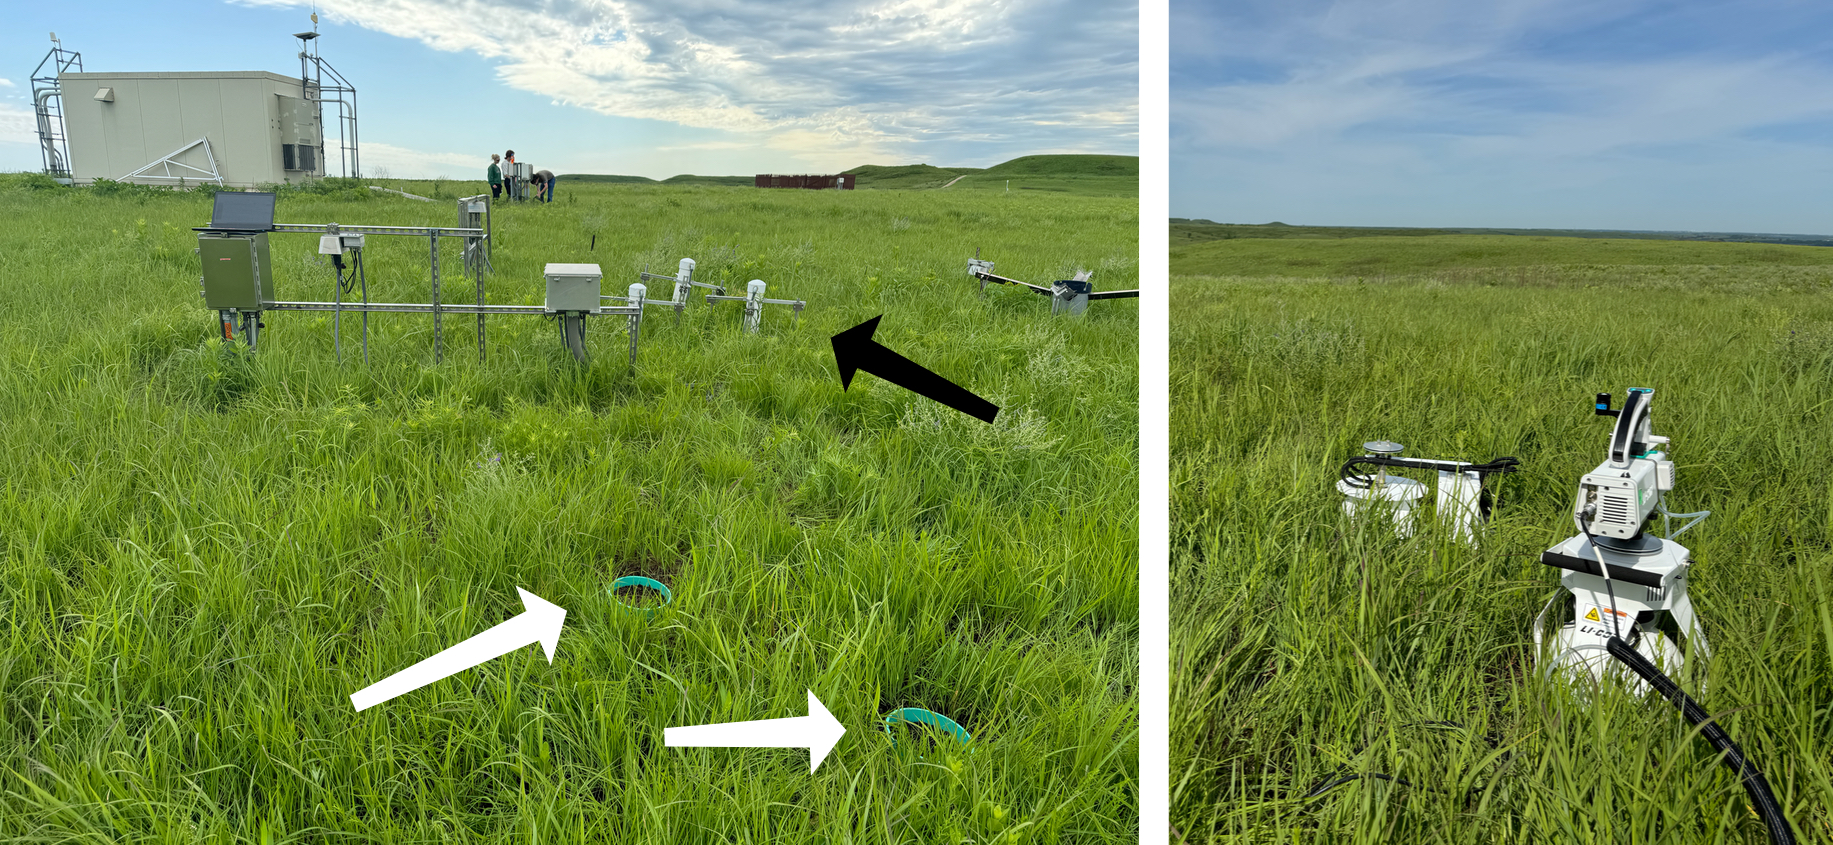
\includegraphics[keepaspectratio]{figures/collar-images.jpeg}}

}

\caption{\label{fig-collar-images}Spatial layout of field sampling using
a closed-dynamic chamber setup at a representative NEON site (KONZ).
Left image shows collars (white arrows) and permanent soil sensor
installation (black arrow) and right image shows the LI-6800
(foreground) and LI-8200-104 (background) instruments placed on the
collars.}

\end{figure}%

\tiny

\begin{longtable}[]{@{}
  >{\raggedright\arraybackslash}p{(\linewidth - 16\tabcolsep) * \real{0.1111}}
  >{\raggedright\arraybackslash}p{(\linewidth - 16\tabcolsep) * \real{0.1111}}
  >{\raggedright\arraybackslash}p{(\linewidth - 16\tabcolsep) * \real{0.1111}}
  >{\raggedright\arraybackslash}p{(\linewidth - 16\tabcolsep) * \real{0.1111}}
  >{\raggedright\arraybackslash}p{(\linewidth - 16\tabcolsep) * \real{0.1111}}
  >{\raggedright\arraybackslash}p{(\linewidth - 16\tabcolsep) * \real{0.1111}}
  >{\raggedright\arraybackslash}p{(\linewidth - 16\tabcolsep) * \real{0.1111}}
  >{\raggedright\arraybackslash}p{(\linewidth - 16\tabcolsep) * \real{0.1111}}
  >{\raggedright\arraybackslash}p{(\linewidth - 16\tabcolsep) * \real{0.1111}}@{}}

\caption{\label{tbl-neon-sites}Listing of NEON sites studied for field
work and analysis. Site refers to NEON site codes: Santa Rita
Experimental Range (SRER), San Joaquin Experimental Range (SJER), Wind
River Experimental Forest (WREF), Chase Lake National Wildlife Refuge
(WOOD), Konza Prairie Biological Station (KONZ), and the University of
Notre Dame Environmental Research Center (UNDE). Location is reported in
decimal degrees of latitude and longitude. Other abbreviations include
Mean Annual Temperature (MAT); \(\overline{T_{S}}\): average soil
temperature during field measurements; \(\overline{SWC}\): average soil
water content during field measurements. Dates refer to field
measurement dates for each site. Plot refers to the particular location
in the soil sensor array (denoted as HOR by NEON) where field
measurements were made.}

\tabularnewline

\toprule\noalign{}
\begin{minipage}[b]{\linewidth}\raggedright
Site
\end{minipage} & \begin{minipage}[b]{\linewidth}\raggedright
Location
\end{minipage} & \begin{minipage}[b]{\linewidth}\raggedright
Ecosystem
\end{minipage} & \begin{minipage}[b]{\linewidth}\raggedright
MAT
\end{minipage} & \begin{minipage}[b]{\linewidth}\raggedright
\(\overline{T_{S}}\)
\end{minipage} & \begin{minipage}[b]{\linewidth}\raggedright
MAP
\end{minipage} & \begin{minipage}[b]{\linewidth}\raggedright
\(\overline{SWC}\)
\end{minipage} & \begin{minipage}[b]{\linewidth}\raggedright
Dates
\end{minipage} & \begin{minipage}[b]{\linewidth}\raggedright
Plot
\end{minipage} \\
\midrule\noalign{}
\endhead
\bottomrule\noalign{}
\endlastfoot
SRER & 31.91068, -110.83549 & Shrubland & 19.3 \(^{\circ}\)C & 47.6
\(^{\circ}\)C & 346 mm & 4.0\% & May 29-- June 1 2022 & 004 \\
SJER & 37.10878, -119.73228 & Oak woodland & 16.4 \(^{\circ}\)C & 41.7
\(^{\circ}\)C & 540 mm & 1.2\% & June 1--4 2022 & 005 \\
WREF & 45.82049, -121.95191 & Evergreen forest & 9.2 \(^{\circ}\)C &
15.3 \(^{\circ}\)C & 2225 mm & 27.2\% & June 7--9 2022 & 001 \\
WOOD & 47.1282, -99.241334 & Restored prairie & 4.9 \(^{\circ}\)C & 14.9
\(^{\circ}\)C & 495 mm & 14.9\% & June 3--9 2024 & 001 \\
KONZ & 39.100774, -96.563075 & Tallgrass prairie & 12.4 \(^{\circ}\)C &
23.4 \(^{\circ}\)C & 870 mm & 23.4\% & May 29-- June 1 2024 & 001 \\
UNDE & 46.23391, -89.537254 & Deciduous forest & 4.3 \(^{\circ}\)C &
13.0 \(^{\circ}\)C & 802 mm & 13.0\% & May 22--25 2024 & 004 \\

\end{longtable}

\normalsize

\subsubsection{Post-collection processing of field
data}\label{post-collection-processing-of-field-data}

We used LI-COR SoilFluxPro software (v 5.3.1) to assess the data after
collection and to inform sampling parameters. We checked appropriateness
of dead band and measurement durations using built-in evaluation tools.
Based on this, the deadband period was set for 30-40 seconds, depending
on the site, and the measurement duration was 180 seconds with a 30
second pre-purge and a 30 second post-purge at most sites, and a 90 sec
pre- and post-purge at sites with higher humidity due to recent
precipitation events. We also assessed the \(R^{2}\) of linear and
exponential model fits to measured CO\(_{2}\) to verify measurement
quality.

\subsection{\texorpdfstring{\texttt{neonSoilFlux} R
package}{neonSoilFlux R package}}\label{sec-nsf-desc}

We developed an R package
(\href{https://CRAN.R-project.org/package=neonSoilFlux}{\texttt{neonSoilFlux}};
Zobitz et al. (2024)) to compute half-hourly soil carbon fluxes and
uncertainties from NEON data. The objective of the \texttt{neonSoilFlux}
package is a unified workflow (Figure~\ref{fig-package-diagram}) for
soil data acquisition and analysis that supplements the existing data
acquisition R package
(\url{https://CRAN.R-project.org/package=neonUtilities}; Lunch et al.
(2025)).

\begin{figure}

\centering{

\pandocbounded{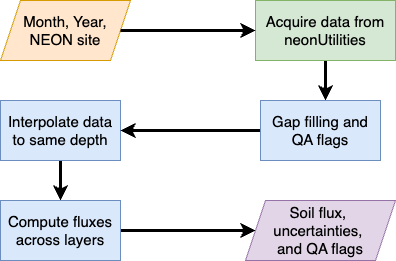
\includegraphics[keepaspectratio]{figures/neonSoilFluxOutline.png}}

}

\caption{\label{fig-package-diagram}Diagram of \texttt{neonSoilFlux} R
package. For a given month, year, and NEON site (orange parallelogram),
the package acquires all relevant data to compute \(F_{S}\) using the
\texttt{neonUtilities} R package (green rectangle). Data are gap-filled
according to reported QA flags and interpolated to the same measurement
depth before computing the soil flux, uncertainties, and final QA flags
(blue rectangles). The package reports the associated soil flux,
uncertainties, and quality assurance (QA) flags for the user (purple
parallelogram).}

\end{figure}%

At a given NEON site there are five replicate soil plots, each with
measurements of soil CO\(_{2}\) concentration, soil temperature, and
soil moisture at different depths (Figure~\ref{fig-model-diagram}). The
\texttt{neonSoilFlux} package acquires measured soil water content
(National Ecological Observatory Network (NEON), 2024e), soil CO\(_{2}\)
concentration (National Ecological Observatory Network (NEON), 2024b),
barometric pressure from the nearby tower (National Ecological
Observatory Network (NEON), 2024a), soil temperature (National
Ecological Observatory Network (NEON), 2024d), and soil properties
(e.g.~bulk density) (National Ecological Observatory Network (NEON),
2024c). The static soil properties were collected from a nearby soil pit
during site characterization and are assumed to be constant at each
site. A soil flux calculation is computed at each replicate soil plot.

\begin{figure}

\centering{

\pandocbounded{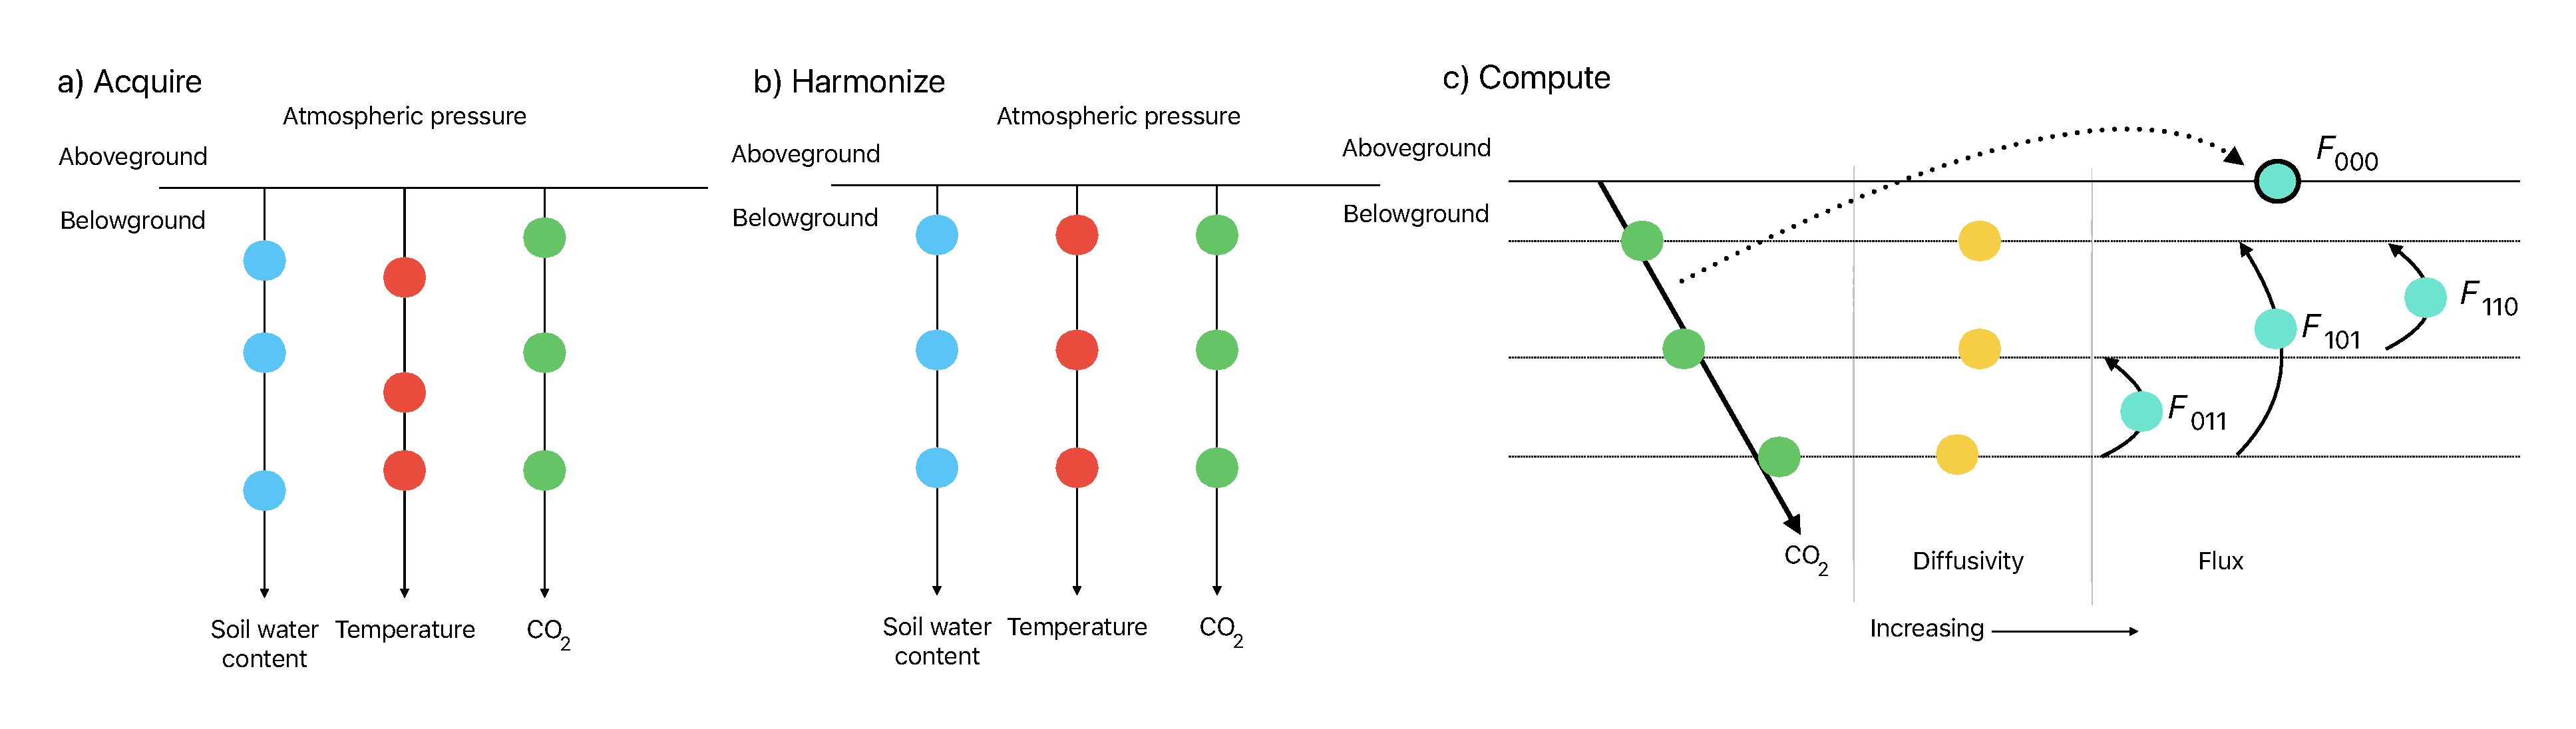
\includegraphics[keepaspectratio]{figures/model-diagram.pdf}}

}

\caption{\label{fig-model-diagram}Model diagram for data workflow for
the \texttt{neonSoilFlux} R package. a) Acquire: Data are obtained from
given NEON location and horizontal sensor location, which includes soil
water content, soil temperature, CO\(_{2}\) concentration, and
atmospheric pressure. All data are screened for quality assurance; if
gap-filling of missing data occurs, it is flagged for the user. b) Any
belowground data are then harmonized to the same depth as CO\(_{2}\)
concentrations using linear regression. c) The flux across a given depth
is computed via Fick's law, denoted with \(F_{ijk}\), where \(i\),
\(j\), or \(k\) are either 0 or 1 denoting the layers the flux is
computed across (\(i\) = closest to surface, \(k\) = deepest).
\(F_{000}\) represents a flux estimate where the gradient \(dC/dz\) is
the slope of a linear regression of CO\(_{2}\) with depth.}

\end{figure}%

The workflow to compute a value of \(F_{S}\) with \texttt{neonSoilFlux}
consists of three primary steps, illustrated in
Figure~\ref{fig-model-diagram}. First, NEON data are acquired for a
given site and month via the \texttt{neonUtilities} R package (yellow
parallelogram and green rectangle in Figure~\ref{fig-package-diagram}
and Panel a in Figure~\ref{fig-model-diagram}). Acquired environmental
data can be exported to a comma separated value file for additional
analysis. Quality assurance (QA) flags are reported as an indicator
variable. Since the calibration coefficients on the soil water content
sensors have changed over time (National Ecological Observatory Network
(NEON), 2024e), raw sensor measurements were back-calculated and
soil-specific calibrations were applied following Ayres et al. (2024) to
generate a consistent time series at each measurement location.

The second step is harmonizing the data to compute soil fluxes across
soil layers. This step consists of three different actions (blue
rectangles in Figure~\ref{fig-package-diagram} and Panel b in
Figure~\ref{fig-model-diagram}). If a given observation by NEON is
reported as not passing a quality assurance check, we applied a gap
filling method to replace that measurement with its monthly mean at that
same depth (Section~\ref{sec-gapfilling}). Belowground measurements of
soil water and soil temperature are then interpolated to the same depth
as soil CO\(_{2}\) measurements. The diffusivity
(Section~\ref{sec-compute-diffusivity}) and soil flux across different
soil layers (Section~\ref{sec-compute-soil-flux}) are then computed.

The third and final step is computing a surface soil flux through
extrapolation to the surface (purple parallelogram in
Figure~\ref{fig-package-diagram} and Panel c in
Figure~\ref{fig-model-diagram}). Uncertainty on a soil flux measurement
is computed through quadrature. An aggregate quality assurance (QA) flag
for each environmental measurement is also reported, representing if any
gap-filled measurements were used in the computation of a soil flux.
Within the soil flux-gradient method, several different approaches can
be used to derive a surface flux (Maier \& Schack-Kirchner, 2014); the
\texttt{neonSoilFlux} package reports four different possible values for
soil surface flux (Section~\ref{sec-compute-soil-flux}).

\subsubsection{Gap-filling routine}\label{sec-gapfilling}

NEON reports QA flags as binary values for each measurement and
half-hourly interval. For a given half-hour, if any input variable (soil
CO\(_2\) concentration, soil temperature, or soil moisture) at depth
\(z\) is flagged, computation of \(F_S\) is not possible. To address
this, flagged measurements and their uncertainties were replaced with a
bootstrapped monthly mean (\(\overline{m}\)) and monthly standard
deviation (\(\overline{s}\)) (Efron \& Tibshirani, 1994).

For each month, depth \(z\), and variable, we computed bootstrapped
estimates of \(\overline{m}\) and \(\overline{s}\) from the vectors of
unflagged measurements (\(\mathbf{m}\)), reported standard errors
(\(\boldsymbol\sigma\)), and the 95\% confidence interval
(\(\boldsymbol\epsilon\), or expanded uncertainty; Farrance \& Frenkel
(2012)). We also defined a bias vector
\(\mathbf{b}=\sqrt{\boldsymbol\epsilon^{2}-\boldsymbol\sigma^{2}}\),
which quantifies the spread of uncertainty in a given period and is
incorporated into \(\overline{m}\).

From these, 5000 bootstrap samples were generated for
\(\mathbf{m}, \boldsymbol\sigma\), and \(\mathbf{b}\). For each sample
(\(m_k, b_k, \sigma_k\)), we generated a vector \(\mathbf{n}\) (length
\(N=5000\)) by drawing from a normal distribution with mean \(m_k+b_k\)
and standard deviation \(\sigma_k\). The sample mean and standard
deviation were then computed from \(\mathbf{n}\). The resulting
distributions of sample means and sample standard deviations provided
the bootstrapped monthly mean (\(\overline{m}\)) and standard error
(\(\overline{s}\)) respectively.

This gap-filling procedure provides a consistent treatment across all
data streams. However, alternative approaches may be better suited for
longer gaps (e.g., correlations with other NEON measurement levels or
soil plots) or for variable-specific conditions. We discuss the effect
of gap-filling on our results in Section~\ref{sec-general-eval}.

\subsubsection{Soil diffusivity}\label{sec-compute-diffusivity}

Soil diffusivity \(D_{a}\) at a given measurement depth is the product
of the diffusivity in free air \(D_{a,0}\) (m\(^{2}\) s\(^{-1}\)) and
the tortuosity \(\xi\) (no units) (Millington \& Shearer, 1971).

We compute \(D_{a,0}\) with Equation \ref{eq:da0}:

\begin{equation}
  D_{a,0} = 0.0000147 \cdot \left( \frac{T_{i} + 273.15}{293.15} \right)^{1.75} \cdot \left( \frac{P}{101.3} \right)
  \label{eq:da0}
\end{equation}

where \(T_{i}\) is soil temperature (\(^\circ\)C) at depth \(i\)
(National Ecological Observatory Network (NEON), 2024d) and \(P\)
surface barometric pressure (kPa) (National Ecological Observatory
Network (NEON), 2024a).

Previous studies by Sallam et al. (1984) and Tang et al. (2003)
demonstrated the sensitivity of modeled \(F_{S}\) depending on the
tortuosity model (\(\xi\)) used to compute diffusivity. At low soil
water content, the choice of tortuosity model can lead to
order-of-magnitude differences in \(D_{a}\), which in turn affect
modeled \(F_{S}\). The \texttt{neonSoilFlux} package currently includes
two approaches to calculate \(\xi\), representing the range of
tortuosity behavior reported in Sallam et al. (1984).

The first approach is the Millington-Quirk model (Millington \& Shearer,
1971), in which tortuosity depends on both porosity and soil water
content:

\begin{equation}
  \xi = \frac{(\phi - SWC_{i})^{10/3}}{\phi^{2}}
  \label{eq:tortuosity-mq}
\end{equation}

In Equation \ref{eq:tortuosity-mq}, \(SWC\) is the soil water content at
depth \(i\) (National Ecological Observatory Network (NEON), 2024e) and
\(\phi\) is the porosity, which in turn is a function of soil physical
properties (National Ecological Observatory Network (NEON), 2024c):

\begin{equation}
  \phi = \left(1- \frac{\rho_{s}}{\rho_{m}} \right) \left(1-f_{V}\right)
  \label{eq:porosity}
\end{equation}

In Equation \ref{eq:porosity}, \(\rho_{m}\) is the particle density of
mineral soil (2.65 g cm\(^{-3}\)), \(\rho_{s}\) the soil bulk density (g
cm\(^{-3}\)) excluding coarse fragments greater than 2 mm (National
Ecological Observatory Network (NEON), 2024c), and \(f_{V}\) is a
site-specific value that accounts for the proportion of soil fragments
between 2-20 mm. Soil fragments greater than 20 mm were not estimated
due to limitations in the amount of soil that can be analyzed (National
Ecological Observatory Network (NEON), 2024c). We assume that rock
fragments contain no internal pores.

The Millington-Quirk model assumes \(\xi\) is modulated by the amount of
fluid saturation in soil pores (Millington \& Shearer, 1971). In
contrast, the Marshall model (Marshall, 1959) expresses tortuosity as
only a function of porosity (\(\xi = \phi^{1.5}\)), with \(\phi\)
defined from Equation \ref{eq:porosity}. The Marshall model is
independent of soil water content and assumes tortuosity is only
governed by soil structure. The \texttt{neonSoilFlux} package allows
users to choose the tortuosity model most appropriate for site-specific
conditions and research goals.

\subsubsection{Soil flux computation}\label{sec-compute-soil-flux}

We applied Fick's law (Equation \ref{eq:ficks}) to compute the soil flux
\(F_{ij}\) (\(\mu\)mol m\(^{-2}\) s\(^{-1}\)) across two soil depths
\(i\) and \(j\):

\begin{equation}
  F_{ij} = -D_{a} \frac{dC}{dz}
  \label{eq:ficks}
\end{equation}

where \(D_{a}\) is the diffusivity (m\(^{2}\) s\(^{-1}\)) and
\(\frac{dC}{dz}\) is the gradient of CO\(_{2}\) molar concentration
(\(\mu\)mol m\(^{-3}\), so the gradient has units of \(\mu\)mol
m\(^{-3}\) m\(^{-1}\)). The soil surface flux is theoretically defined
by applying Equation \ref{eq:ficks} to measurements collected at the
soil surface and directly below the surface. Measurements of soil
temperature, soil water content, and soil CO\(_{2}\) molar concentration
across the soil profile allow for application of Equation \ref{eq:ficks}
across different soil depths. Each site had three measurement layers, so
we denote the flux as a three-digit subscript \(F_{ijk}\) with indicator
variables \(i\), \(j\), and \(k\) indicate if a given layer was used
(written in order of increasing depth), according to the following:

\begin{itemize}
\tightlist
\item
  \(F_{000}\) is a surface flux estimate using the intercept of the
  linear regression of \(D_{a}\) with depth and the slope from the
  linear regression of CO\(_{2}\) with depth (which represents
  \(\displaystyle \frac{dC}{dz}\) in Fick's Law). Tang et al. (2003)
  used this approach to compute fluxes in an oak-grass savannah.
\item
  \(F_{110}\), \(F_{011}\) are fluxes across the two most shallow layers
  and two deepest layers respectively. The diffusivity used in Fick's
  Law is always at the deeper measurement layer. When used as a surface
  flux estimate we assume CO\(_{2}\) remains constant above this flux
  depth.
\item
  \(F_{101}\) is a surface flux estimate using linear extrapolation
  using concentration measurements between the shallowest and deepest
  measurement layer. Hirano et al. (2003) and Tang et al. (2005) used an
  approach similar to \(F_{101}\) in a temperate deciduous broadleaf
  forest and ponderosa pine forest respectively.
\end{itemize}

Uncertainty in all \(F_{ijk}\) is computed through quadrature (Taylor,
2022).

\subsection{Post processing evaluation}\label{sec-post-process}

Following collection of field measurements and calculation of the soil
fluxes from \texttt{neonSoilFlux} package, we compared measured
\(F_{S}\) based on closed-dynamic chamber measurements with the LI-COR
instruments to a given soil flux calculation from \texttt{neonSoilFlux}
for each site and flux computation method. Statistics included the ,
slope from a linear regression (\(m\)), normalized root mean squared
error (NRMSE), and associated R\(^{2}\) value.

Finally, for a half-hourly interval we also computed a \emph{post hoc}
\(D_{a}\) using the LI-COR flux along with the CO\(_{2}\) surface
gradient reported by NEON using the measurement levels closest to the
surface.

\section{Results}\label{results}

\subsection{\texorpdfstring{Concordance between modelled and measured
soil CO\(_{2}\)
flux}{Concordance between modelled and measured soil CO\_\{2\} flux}}\label{concordance-between-modelled-and-measured-soil-co_2-flux}

The sites we visited ranged substantially in both their annual average
temperature and precipitation as well as their biome type
(Table~\ref{tbl-licor-results}). These differences also influenced the
wide range of observed flux rates across sites.

\begin{table}

\caption{\label{tbl-licor-results}Summary of measured soil
characteristics and flux results from field measurements across six NEON
sites using a LI-COR 6800 (LI-870/8250 measurements omitted to enable
direct comparability) via the closed-dynamic chamber method. Numeric
values for soil CO\(_{2}\) flux, soil temperature, and volumetric soil
water content (VSWC) are the mean and standard deviation of field
measurements at each site.}

\centering{

\begin{tabular}{ccccc}
\toprule
Site & \makecell[c]{Flux\\ $\mu$mol m$\textsuperscript{-2}$ s$\textsuperscript{-1}$} & \makecell[c]{Soil temp\\ °C} & \makecell[c]{VSWC\\ cm$\textsuperscript{3}$ cm$\textsuperscript{-3}$} & n\\
\midrule
UNDE & 2.55 $\pm$ 0.26 & 14.33 $\pm$ 0.77 & 0.33 $\pm$ 0.02 & 61\\
WOOD & 3.02 $\pm$ 0.4 & 16.01 $\pm$ 1.54 & 0.28 $\pm$ 0.01 & 53\\
WREF & 3.62 $\pm$ 0.3 & 15.34 $\pm$ 1.76 & 0.27 $\pm$ 0.06 & 21\\
KONZ & 6.35 $\pm$ 0.97 & 27.28 $\pm$ 4.14 & 0.37 $\pm$ 0.01 & 44\\
SJER & 0.94 $\pm$ 0.02 & 41.68 $\pm$ 11.22 & 0.01 $\pm$ 0.01 & 32\\
SRER & 0.72 $\pm$ 0.09 & 47.64 $\pm$ 7.46 & 0.04 $\pm$ 0.01 & 32\\
\bottomrule
\end{tabular}

}

\end{table}%

The timeseries of the measured fluxes from the LI-COR 6800 and 870/8250
were compared to modeled soil fluxes from the \texttt{neonSoilFlux} R
package (Figure~\ref{fig-flux-results}). We also assessed year-long
estimated flux time series and compared those to field measurements made
at each site (Figure~\ref{fig-flux-results-year}). Results are reported
in local time. Where applicable, sites are displayed from left to right
by increasing soil temperature (Table~\ref{tbl-neon-sites}). Positive
values of the flux indicate that there is a flux moving towards the
surface. Overall, with the exception of SRER (discussed later) the
computed fluxes determined using a variety of plausible methods spanned
the field-measured fluxes, but the specific flux-gradient method that
best approximated field measurements varied by site.

\begin{figure}

\centering{

\pandocbounded{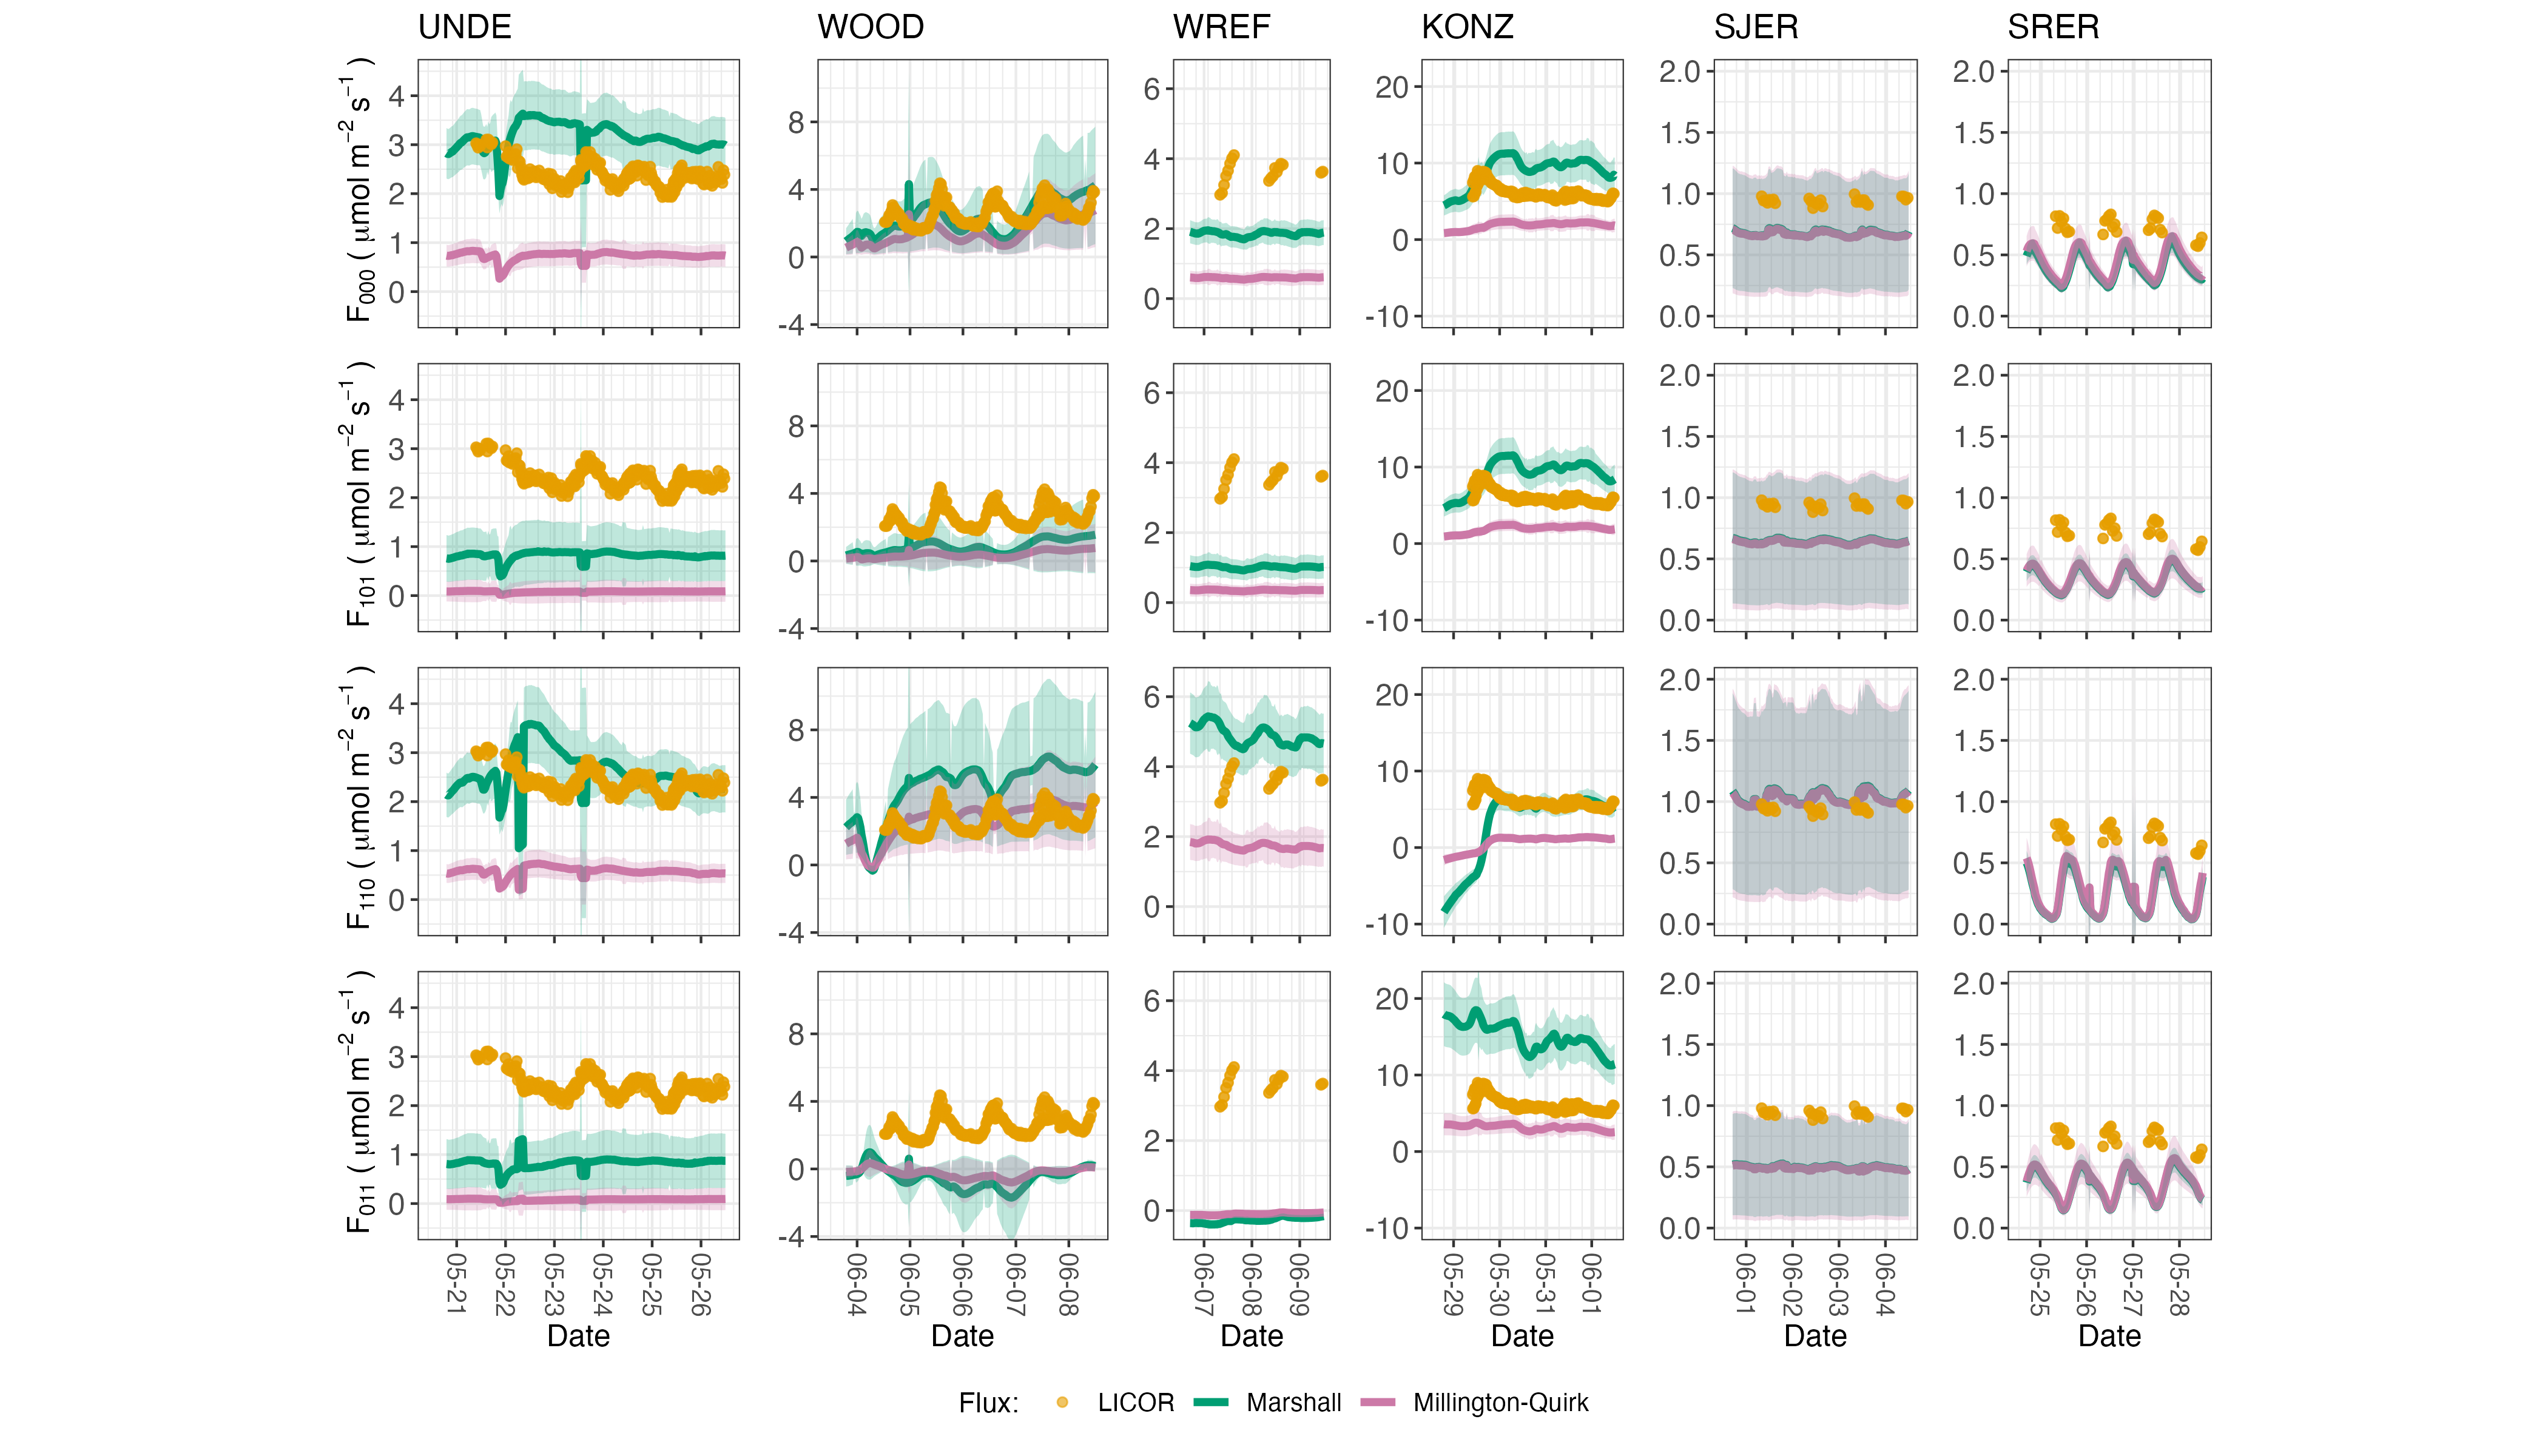
\includegraphics[keepaspectratio]{figures/flux-results.png}}

}

\caption{\label{fig-flux-results}Timeseries of soil surface flux
(\(F_{S}\)) from LICOR measured (yellow lines) and modeled soil fluxes
(green or purple lines) by the \texttt{neonSoilFlux} R package. Fluxes
from the \texttt{neonSoilFlux} R package are separated by the
diffusivity model used (Millington-Quirk or Marshall,
Section~\ref{sec-compute-diffusivity}). Individual vertical axis labels
in the first column represent the measurement levels where the
flux-gradient approach is applied (Section~\ref{sec-compute-soil-flux}).
Ribbons for modeled soil fluxes represent \(\pm\) 1 standard deviation.
Results are reported in local time.}

\end{figure}%

\begin{figure}

\centering{

\pandocbounded{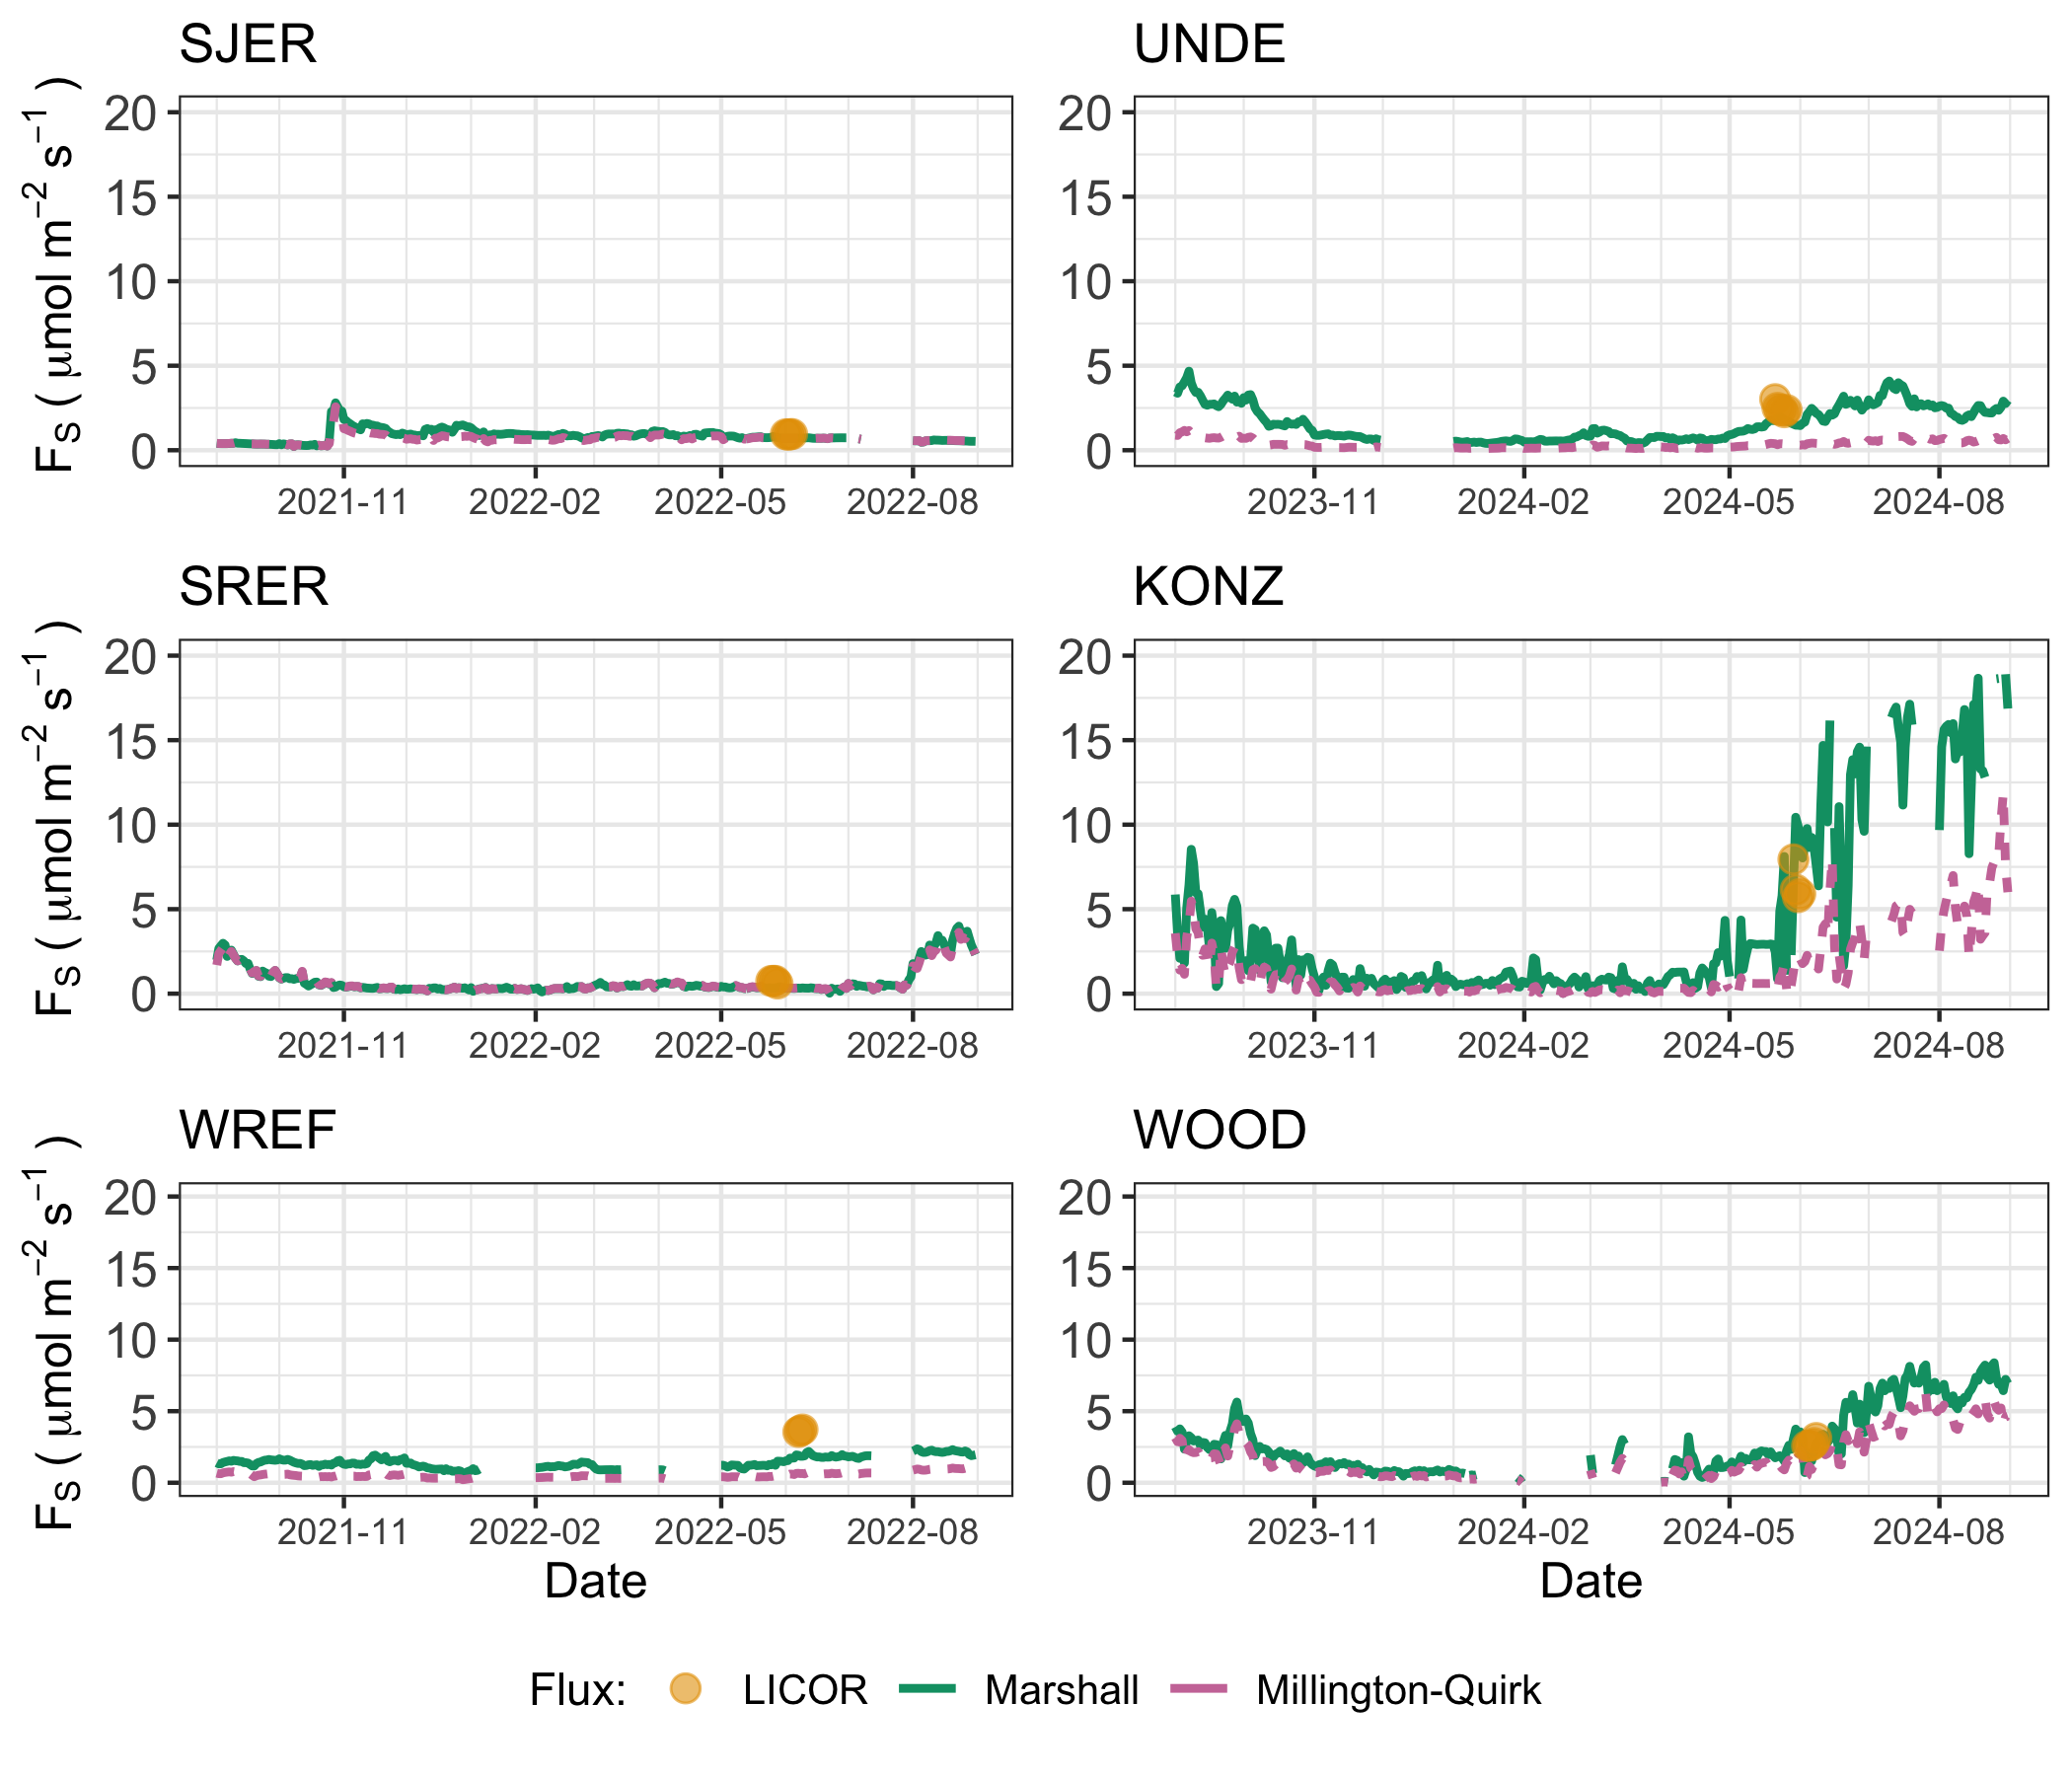
\includegraphics[keepaspectratio]{figures/flux-results-year.png}}

}

\caption{\label{fig-flux-results-year}Timeseries of both daily-averaged
field \(F_{S}\) (yellow circles) and daily ensemble averaged soil fluxes
(average of \(F_{000}\), \(F_{101}\), \(F_{011}\), \(F_{110}\),
Section~\ref{sec-compute-soil-flux}) by the \texttt{neonSoilFlux} R
package, separated by the diffusivity model used (green or purple lines,
Millington-Quirk or Marshall, Section~\ref{sec-compute-diffusivity}).}

\end{figure}%

We calculated the statistical 1-1 comparison between the various
estimates of soil flux computed by \texttt{neonSoilFlux} with the
field-measured fluxes within half-hourly periods. Statistics for these
comparisons are reported in Table~\ref{tbl-flux-11-compare}.

\begin{table}

\caption{\label{tbl-flux-11-compare}Statistical comparison between
measured fluxes at each site with fluxes reported by
\texttt{neonSoilFlux} with the different diffusivity calculations
applied. \emph{m} refers to the slope of a linear regression between the
LICOR measured fluxes at each site and the outputs from
\texttt{neonSoilFlux}. * = significance at the 5\% level, ** =
significance at the 1\% level. NRMSE is the normalized root mean square
error between measured and \texttt{neonSoilFlux} outputs, normalized by
the sample mean of the LICOR measured fluxes.}

\centering{

\pandocbounded{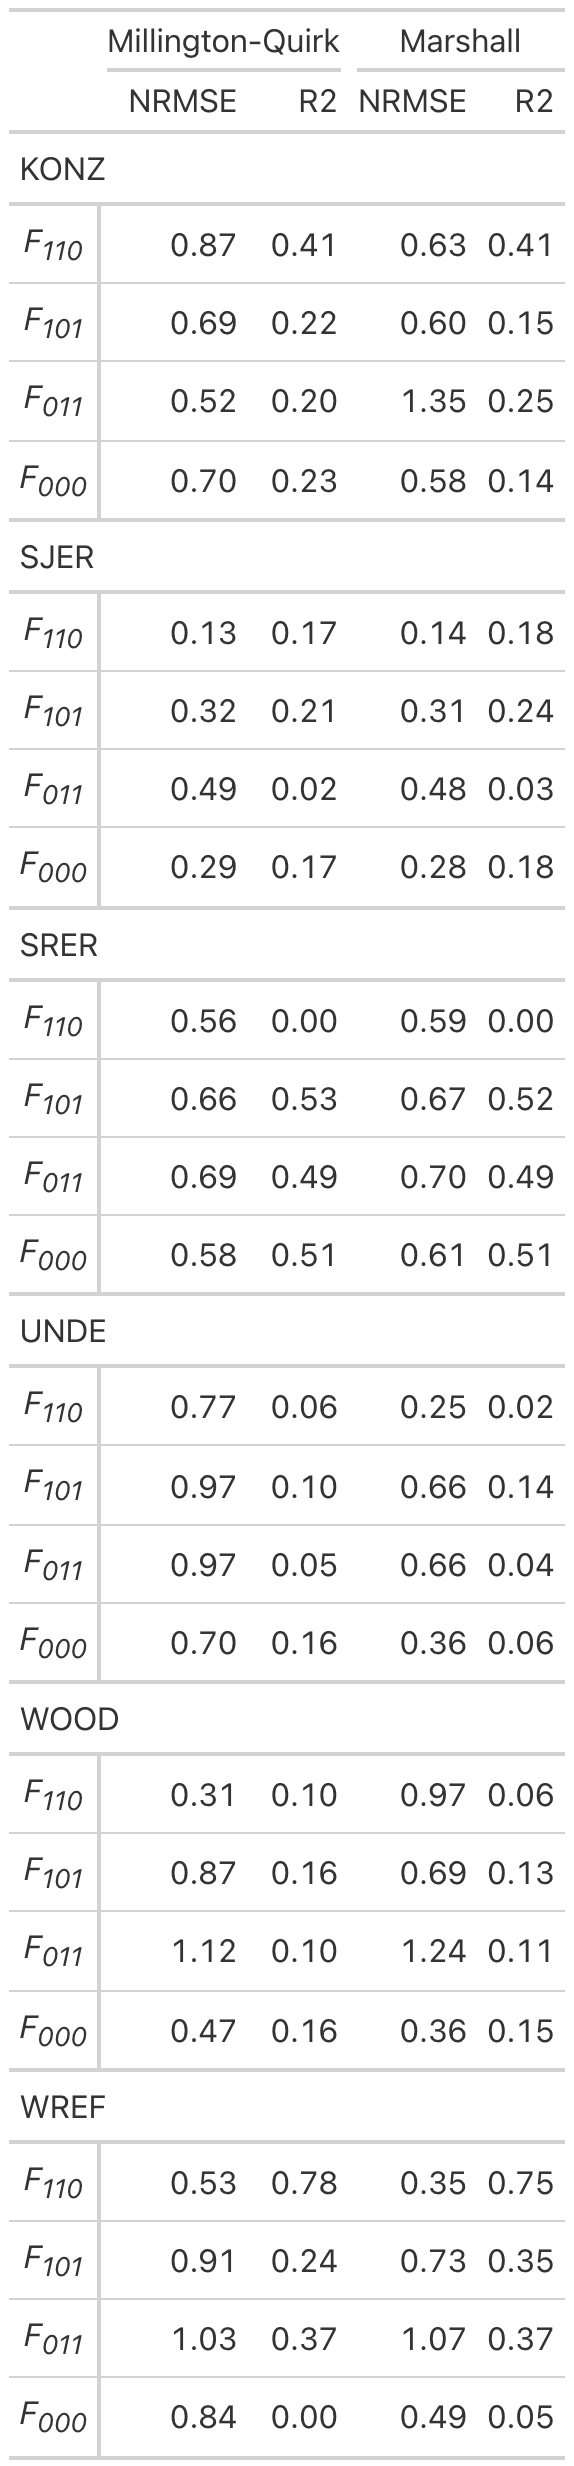
\includegraphics[keepaspectratio]{figures/r2-plot.png}}

}

\end{table}%

\subsection{Effects of method choice on diffusivity
estimates}\label{effects-of-method-choice-on-diffusivity-estimates}

In four of six field sites, the \emph{post hoc} \(D_{a}\) estimate fell
roughly between the two diffusion estimation methods; however this was
less the case in the two driest sites, SJER and SRER
(Table~\ref{tbl-neon-sites}), where the field estimate of diffusivity
was either lower or higher than both of the other methods
(Figure~\ref{fig-diffusivity-plot}).

\begin{figure}

\centering{

\pandocbounded{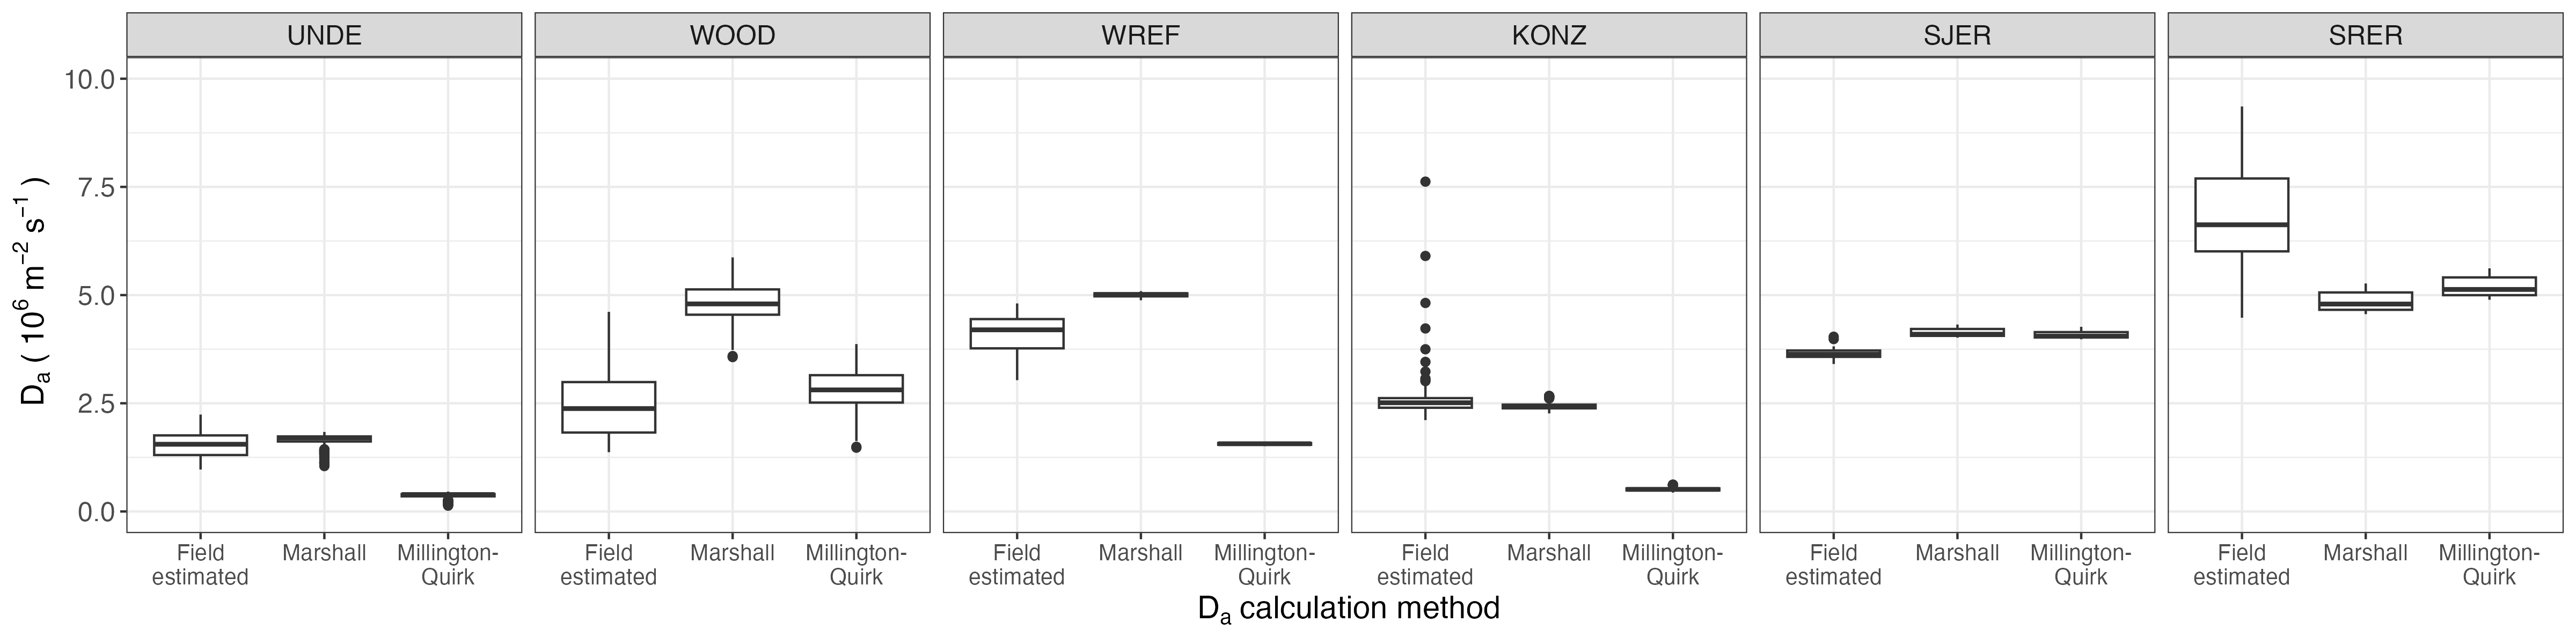
\includegraphics[keepaspectratio]{figures/diffusivity-plot.png}}

}

\caption{\label{fig-diffusivity-plot}Distribution of diffusivity
(\(D_{a}\)) at each study site. Values of \(D_{a}\) were provided by the
\texttt{neonSoilFlux} package, computed from the Millington-Quirk or
Marshall models (Section~\ref{sec-compute-diffusivity}). A post-hoc
estimate of diffusivity (labeled as ``Field estimated'') was computed
through the field measured flux (Figure~\ref{fig-flux-results}), divided
by the CO\(_{2}\) gradient from the measurement levels closest to the
soil surface, as reported by NEON. We only used \(F_{S}\) measured by
the LICOR 6800 at all sites to standardize comparisons.}

\end{figure}%

\section{Discussion}\label{sec-discussion}

This study presents a unified data science workflow to efficiently
process automated measurements of belowground soil CO\(_{2}\)
concentrations, soil water content, and soil temperature to infer
estimates of soil surface CO\(_{2}\) effluxes through application of
Fick's Law (Equation \ref{eq:ficks}). Our core goals in this study were:
(1) to generate estimates of soil flux from continuous soil sensor data
at terrestrial NEON sites using the flux-gradient method and then (2) to
compare those estimates to field-measured fluxes based on the closed
chamber approach at six NEON focal sites. We discuss our progress toward
these core goals through (1) an overall evaluation of the flux-gradient
approach (and uncertainty calculation) and (2) site-specific evaluation
of differences in estimated vs measured fluxes.

\subsection{General evaluation of flux-gradient
approach}\label{sec-general-eval}

Key assumptions of the flux-gradient approach are that CO\(_{2}\)
concentrations increase throughout the soil profile such that the
highest concentrations are observed in the deepest layers. Additionally,
field flux measurements should correlate with \(F_{000}\) because they
represent surface fluxes. Periods where this gradient condition are not
met generally are connected to processes that occur during soil wetting
events, where more shallow soil layers produce higher concentrations of
CO\(_{2}\) due to microbial respiration pulses following rewetting. This
effect is likely to be largest at sites with rich organic soils
(e.g.~KONZ). Based on this reasoning, in these types of situations we
would \emph{a priori} expect
\(F_{011} \mbox{ (deepest layers) } \leq F_{101} \leq F_{110} \mbox{ (shallow layers) } \leq F_{000} \mbox{ (all layers) }\)
because the previous flux estimates rely primarily on CO\(_2\)
concentrations at deeper depths, and could miss high concentrations of
CO\(_{2}\) produced in shallower layers.

When modeling soil respiration, typically a non-linear response function
that also considers soil type is used (Bouma \& Bryla, 2000; Yan et al.,
2016, 2018). For the \texttt{neonSoilFlux} package, soil type is
connected to the measurement of bulk density, which was characterized at
each NEON site. This bulk density estimate is based on replicate samples
collected from the site megapit at a subset of soil horizons, with an
estimated uncertainty of \(\pm5\%\) (National Ecological Observatory
Network (NEON), 2024c). Coarse fragment estimates also have very large
uncertainties, but because the volume fraction tends to be low in
surface soils it probably wouldn't contribute much additional flux
uncertainty.

Our results suggest that the most important way to improve reliability
of the flux estimate is to reduce the usage of gap-filled data. The
current approach to gap filling in \texttt{neonSoilFlux} uses monthly
mean data to gap fill---this approach decreases the ability of the
estimate to be responsive to short-term pulses that occur with rapid
weather shifts. Four sites (KONZ, SRER, WREF, and UNDE) had more than
75\% of half-hourly periods with no-gap filled measurements (Figure S1,
Supplementary Information). Two sites (SJER and WOOD) had more than 75\%
of half-hourly intervals with just one gap-filled measurement. While we
did not need to use gap-filled measurements to compute the flux at WREF,
field data collection occurred following a severe rainstorm, with soils
at the beginning of the sampling week near their water holding capacity.
We recommend that whenever possible, knowledge of local field conditions
should influence analysis decisions in addition to any QA filtering
protocols in the \texttt{neonSoilFlux} package.

We recognize that this gap-filling approach may lead to gap-filled
values that are quite different from the actual values, such as an
underestimate of soil moisture following rain events. Further extensions
of the gap filling method could use more sophisticated gap-filling
routines, similar to what is used for net ecosystem carbon exchange
(Falge et al., 2001; Liu et al., 2023; Mariethoz et al., 2015; Moffat et
al., 2007; Zhang et al., 2023). The current gap-filling routine provides
a consistent approach that can be applied to each data stream, but
further work may explore alternative gap-filling approaches.

\subsection{Evaluation of flux-gradient approach at each
site}\label{evaluation-of-flux-gradient-approach-at-each-site}

Derived results from the \texttt{neonSoilFlux} package have patterns
that are broadly consistent with those directly measured in the field
(Figure~\ref{fig-flux-results} and Figure~\ref{fig-flux-results-year}),
even though statistical comparisons between the field-measured and
\texttt{neonSoilFlux} values were quite variable and poor
(e.g.~\(R^{2}\) ranging from 0.00 to 0.78;
Table~\ref{tbl-flux-11-compare}). One advantage of the
\texttt{neonSoilFlux} package is its ability to calculate fluxes across
different soil depths (Figure~\ref{fig-model-diagram}), which allows for
additional site-specific customization. We believe the package can
provide a useful baseline estimate of soil fluxes that can always be
complemented through additional field measurements.

The six locations studied provide a range of case studies that suggest
different considerations may apply to different sites when applying the
flux-gradient method. For example, the Santa Rita Experimental Range
(SRER) is a desert site characterized by sandy soil, which also was the
location of the highest field soil temperatures that we observed
(Table~\ref{tbl-licor-results}). At SRER the flux across the top two
layers (\(F_{110}\)) produced a pattern of soil flux most consistent
with the observed field data. The remaining methods \(F_{101}\),
\(F_{011}\), or \(F_{000}\) are derived from information taken from the
deepest layer, which seems to have been decoupled from the surface
layers both in terms of temperature and CO\(_{2}\) concentration. This
may be a general circumstance where there are large diurnal temperature
extremes that rapidly change during the course of a day and overnight,
leading to lags in the timing of when temperature increases propagate
down to deeper soil layers.

Immediately prior to our visit to Konza Prarie (KONZ), that site that
experienced a significant rain event that led to wet soils that
gradually dried out over the course of our time there. This pulse of
precipitation increased the soil CO\(_{2}\) concentration at the top
layer above the concentrations in lower layers, leading to negative
estimated flux values at the start of the experiment. In this case it
was only when the soil began to return to a baseline level that the
assumptions of the flux-gradient method were again met.

Both of the previous cases also provide context for the poor statistical
comparisons between field-measured soil fluxes and \texttt{neonSoilFlux}
outputs Table~\ref{tbl-flux-11-compare}. When considering systematic
deployment of this method across a measurement network, there are a
number of independent challenges that require careful consideration.
There are clear tradeoffs between (1) accuracy of modeled fluxes
(defined here as closeness to field-measured \(F_{S}\) and the
uncertainty reduction factor \(\epsilon\)), (2) precision (which could
be defined by the signal to noise ratio), and (3) the choice of the
diffusivity model (Section~\ref{sec-compute-diffusivity}) or flux
computation method (Section~\ref{sec-compute-soil-flux}). A sensitivity
analysis (Figure S2, Supplemental Information) found that flux output
uncertainty was dominated by measurement uncertainty (\(T_{S}\), \(P\),
\(SWC\), or CO\(_{2}\)) rather than the diffusivity method to compute
soil flux. Notably, the \(F_{110}\) method was least sensitivty to
measurement uncertainty likely because it best aligns with surface
chamber measurement assumptions.

Finally, comparing the effects of different diffusivity estimation
methods on the match between modeled and measured fluxes
(Figure~\ref{fig-flux-results-year}) highlights the sensitivity of
\(F_{ijk}\) to diffusivity. The comparison between diffusivity estimates
compared to field estimated diffusivity
(Figure~\ref{fig-diffusivity-plot}) demonstrates that site parameters
can dictate which measure of diffusivity is most likely to be accurate
in a given environmental context. Site-specific differences a largely a
reflection of differences in soil moisture across the sites
(Table~\ref{tbl-neon-sites}), as not all diffusivity estimation methods
incorporate soil moisture equivalently. While we here have compares two
approaches to calculate diffusivity (the Millington-Quirk and Marshall
models), it may be valuable to evaluate other diffusivity models
(e.g.~the Moldrup model; Moldrup et al. (1999)) as well. Ultimately the
choice of a particular diffusivity model could be determined based on
knowledge of site-specific evaluations or a set of these models could be
used to generate a model ensemble average as a means to trade precision
for a more general approach.

\subsection{Recommendations for future method
development}\label{recommendations-for-future-method-development}

The \texttt{neonSoilFlux} package provides several approaches to
estimate soil flux using the gradient method. We believe these
approaches enable the software to be used across a range of
site-specific assumptions (Maier \& Schack-Kirchner, 2014). We note,
however, that this choice can have a determinative approach on the
calculated values. Ensemble averaging approaches (Elshall et al., 2018;
Raftery et al., 2005) may be one way to address this problem if the goal
is to calculate fluxes using the same method at a diverse range of
different sites. Two other ideas would be to apply machine learning
algorithms (e.g.~random forests) to generate a single flux estimate
across diverse sites, or using co-located estimates of net ecosystem
carbon exchange from eddy-flux towers to further constrain results or to
assess soil flux results for plausibility (Phillips et al., 2017).

These challenges notwithstanding, the method used here and made
available in the \texttt{neonSoilFlux} R package has the potential to
produce nearly continuous estimates of flux across all terrestrial NEON
sites. These estimates are a significant improvement on available
approaches to constrain the portion of ecosystem respiration
attributable to the soil. This, in turn, also aids in our ability to
understand the soil contribution to the net ecosystem flux measured at
these sites using the co-located eddy flux towers.

\section{Conclusions}\label{conclusions}

We used the R package \texttt{neonSoilFlux} to test its broader
application in estimating soil CO\(_2\) fluxes with the flux-gradient
method, using data from continuous buried soil sensors at NEON
terrestrial sites. We compared the predicted fluxes to those measured
directly using a field-based closed chamber approach. Soil fluxes from
\texttt{neonSoilFlux} were broadly effective at producing estimates of
flux comparable to those measured in the field using a chamber-based
technique. However \texttt{neonSoilFlux} outputs are quite sensitive to
a number of issues, including: missing data (and thus gap-filling of
input measurement datasets), the selection of soil depths used to best
calculate the gradient (which may vary between sites), and finally the
choice of method used for estimating soil diffusivity. The flexibility
of the \texttt{neonSoilFlux} package allows the user to evaluate each of
these issues with site-specific knowledge and contexts. Future
refinements and subsequent validation of \texttt{neonSoilFlux} outputs
will feed forward into evaluating soil carbon fluxes broader spatial
scales to enhance understanding of the ways in which soils across
diverse ecosystems are responding to a changing climate.

\section*{Sources Cited}\label{sources-cited}
\addcontentsline{toc}{section}{Sources Cited}

\phantomsection\label{refs}
\begin{CSLReferences}{1}{0}
\bibitem[\citeproctext]{ref-ayresValidationRemotelySensed2024}
Ayres, E., Reichle, R. H., Colliander, A., Cosh, M. H., \& Smith, L.
(2024). Validation of {Remotely Sensed} and {Modeled Soil Moisture} at
{Forested} and {Unforested NEON Sites}. \emph{IEEE Journal of Selected
Topics in Applied Earth Observations and Remote Sensing}, \emph{17},
14248--14264. \url{https://doi.org/10.1109/JSTARS.2024.3430928}

\bibitem[\citeproctext]{ref-baldocchiMeasuringFluxesTrace2014}
Baldocchi, D. (2014). Measuring fluxes of trace gases and energy between
ecosystems and the atmosphere - the state and future of the eddy
covariance method. \emph{Global Change Biology}, \emph{20}(12),
3600--3609. \url{https://doi.org/10.1111/gcb.12649}

\bibitem[\citeproctext]{ref-berenbaumReportNSFBIO2015}
Berenbaum, M. R., Carpenter, S. R., Hampton, S. E., Running, S. W., \&
Stanzione, D. C. (2015). \emph{Report from the {NSF BIO Advisory
Committee Subcommittee} on {NEON Scope Impacts}}.

\bibitem[\citeproctext]{ref-bond-lambertyNewTechniquesData2018}
Bond-Lamberty, B. (2018). New {Techniques} and {Data} for
{Understanding} the {Global Soil Respiration Flux}. \emph{Earth's
Future}, \emph{6}(9), 1176--1180.
\url{https://doi.org/10.1029/2018EF000866}

\bibitem[\citeproctext]{ref-bond-lambertyTwentyYearsProgress2024}
Bond-Lamberty, B., Ballantyne, A., Berryman, E., Fluet-Chouinard, E.,
Jian, J., Morris, K. A., Rey, A., \& Vargas, R. (2024). Twenty {Years}
of {Progress}, {Challenges}, and {Opportunities} in {Measuring} and
{Understanding Soil Respiration}. \emph{Journal of Geophysical Research:
Biogeosciences}, \emph{129}(2), e2023JG007637.
\url{https://doi.org/10.1029/2023JG007637}

\bibitem[\citeproctext]{ref-bond-lambertyCOSORECommunityDatabase2020}
Bond-Lamberty, B., Christianson, D. S., Malhotra, A., Pennington, S. C.,
Sihi, D., AghaKouchak, A., Anjileli, H., Altaf Arain, M., Armesto, J.
J., Ashraf, S., Ataka, M., Baldocchi, D., Andrew Black, T., Buchmann,
N., Carbone, M. S., Chang, S.-C., Crill, P., Curtis, P. S., Davidson, E.
A., \ldots{} Zou, J. (2020). {COSORE}: {A} community database for
continuous soil respiration and other soil-atmosphere greenhouse gas
flux data. \emph{Global Change Biology}, \emph{26}(12), 7268--7283.
\url{https://doi.org/10.1111/gcb.15353}

\bibitem[\citeproctext]{ref-bond-lambertyGlobalDatabaseSoil2010}
Bond-Lamberty, B., \& Thomson, A. (2010). A global database of soil
respiration data. \emph{Biogeosciences}, \emph{7}(6), 1915--1926.
\url{https://doi.org/10.5194/bg-7-1915-2010}

\bibitem[\citeproctext]{ref-bond-lambertyGlobalRelationshipHeterotrophic2004}
Bond-Lamberty, B., Wang, C., \& Gower, S. T. (2004). A global
relationship between the heterotrophic and autotrophic components of
soil respiration? \emph{Global Change Biology}, \emph{10}(10),
1756--1766. \url{https://doi.org/10.1111/j.1365-2486.2004.00816.x}

\bibitem[\citeproctext]{ref-boumaAssessmentRootSoil2000}
Bouma, T. J., \& Bryla, D. R. (2000). On the assessment of root and soil
respiration for soils of different textures: Interactions with soil
moisture contents and soil {CO2} concentrations. \emph{Plant and Soil},
\emph{227}(1), 215--221. \url{https://doi.org/10.1023/A:1026502414977}

\bibitem[\citeproctext]{ref-chenDoesGeneralTemperatureDependent2005}
Chen, H., \& Tian, H.-Q. (2005). Does a {General Temperature-Dependent
Q10 Model} of {Soil Respiration Exist} at {Biome} and {Global Scale}?
\emph{Journal of Integrative Plant Biology}, \emph{47}(11), 1288--1302.
\url{https://doi.org/10.1111/j.1744-7909.2005.00211.x}

\bibitem[\citeproctext]{ref-davidsonVariabilityRespirationTerrestrial2006}
Davidson, E. A., Janssens, I. A., \& Luo, Y. (2006). On the variability
of respiration in terrestrial ecosystems: Moving beyond {Q10}.
\emph{Global Change Biology}, \emph{12}, 154--164.
\url{https://doi.org/10.1111/j.1365-2486.2005.01065.x}

\bibitem[\citeproctext]{ref-desaiDriversDecadalCarbon2022}
Desai, A. R., Murphy, B. A., Wiesner, S., Thom, J., Butterworth, B. J.,
Koupaei-Abyazani, N., Muttaqin, A., Paleri, S., Talib, A., Turner, J.,
Mineau, J., Merrelli, A., Stoy, P., \& Davis, K. (2022). Drivers of
{Decadal Carbon Fluxes Across Temperate Ecosystems}. \emph{Journal of
Geophysical Research: Biogeosciences}, \emph{127}(12), e2022JG007014.
\url{https://doi.org/10.1029/2022JG007014}

\bibitem[\citeproctext]{ref-efronIntroductionBootstrap1994}
Efron, B., \& Tibshirani, R. J. (1994). \emph{An {Introduction} to the
{Bootstrap}}. {Chapman and Hall/CRC}.
\url{https://doi.org/10.1201/9780429246593}

\bibitem[\citeproctext]{ref-elshallRelativeModelScore2018}
Elshall, A. S., Ye, M., Pei, Y., Zhang, F., Niu, G.-Y., \&
Barron-Gafford, G. A. (2018). Relative model score: A scoring rule for
evaluating ensemble simulations with application to microbial soil
respiration modeling. \emph{Stochastic Environmental Research and Risk
Assessment}, \emph{32}(10), 2809--2819.
\url{https://doi.org/10.1007/s00477-018-1592-3}

\bibitem[\citeproctext]{ref-falgeGapFillingStrategies2001}
Falge, E., Baldocchi, D., Olson, R., Anthoni, P., Aubinet, M.,
Bernhofer, C., Burba, G., Ceulemans, R., Clement, R., Dolman, H.,
Granier, A., Gross, P., Grünwald, T., Hollinger, D., Jensen, N.-O.,
Katul, G., Keronen, P., Kowalski, A., Lai, C. T., \ldots{} Wofsy, S.
(2001). Gap filling strategies for defensible annual sums of net
ecosystem exchange. \emph{Agricultural and Forest Meteorology},
\emph{107}(1), 43--69.
\url{https://doi.org/10.1016/S0168-1923(00)00225-2}

\bibitem[\citeproctext]{ref-farranceUncertaintyMeasurementReview2012}
Farrance, I., \& Frenkel, R. (2012).
\href{https://www.ncbi.nlm.nih.gov/pmc/articles/PMC3387884}{Uncertainty
of {Measurement}: {A Review} of the {Rules} for {Calculating Uncertainty
Components} through {Functional Relationships}}. \emph{The Clinical
Biochemist Reviews}, \emph{33}(2), 49--75.

\bibitem[\citeproctext]{ref-friedlingsteinGlobalCarbonBudget2025}
Friedlingstein, P., O'Sullivan, M., Jones, M. W., Andrew, R. M., Hauck,
J., Landschützer, P., Le Quéré, C., Li, H., Luijkx, I. T., Olsen, A.,
Peters, G. P., Peters, W., Pongratz, J., Schwingshackl, C., Sitch, S.,
Canadell, J. G., Ciais, P., Jackson, R. B., Alin, S. R., \ldots{} Zeng,
J. (2025). Global {Carbon Budget} 2024. \emph{Earth System Science
Data}, \emph{17}(3), 965--1039.
\url{https://doi.org/10.5194/essd-17-965-2025}

\bibitem[\citeproctext]{ref-hamdiSynthesisAnalysisTemperature2013}
Hamdi, S., Moyano, F., Sall, S., Bernoux, M., \& Chevallier, T. (2013).
Synthesis analysis of the temperature sensitivity of soil respiration
from laboratory studies in relation to incubation methods and soil
conditions. \emph{Soil Biology and Biochemistry}, \emph{58}, 115--126.
\url{https://doi.org/10.1016/j.soilbio.2012.11.012}

\bibitem[\citeproctext]{ref-hiranoLongtermHalfhourlyMeasurement2003}
Hirano, T., Kim, H., \& Tanaka, Y. (2003). Long-term half-hourly
measurement of soil {CO2} concentration and soil respiration in a
temperate deciduous forest. \emph{Journal of Geophysical Research:
Atmospheres}, \emph{108}(D20).
\url{https://doi.org/10.1029/2003JD003766}

\bibitem[\citeproctext]{ref-jacksonEcologySoilCarbon2017}
Jackson, R. B., Lajtha, K., Crow, S. E., Hugelius, G., Kramer, M. G., \&
Piñeiro, G. (2017). The {Ecology} of {Soil Carbon}: {Pools},
{Vulnerabilities}, and {Biotic} and {Abiotic Controls}. \emph{Annual
Review of Ecology, Evolution and Systematics}, \emph{48}(Volume 48,
2017), 419--445.
\url{https://doi.org/10.1146/annurev-ecolsys-112414-054234}

\bibitem[\citeproctext]{ref-jianHistoricallyInconsistentProductivity2022}
Jian, J., Bailey, V., Dorheim, K., Konings, A. G., Hao, D., Shiklomanov,
A. N., Snyder, A., Steele, M., Teramoto, M., Vargas, R., \&
Bond-Lamberty, B. (2022). Historically inconsistent productivity and
respiration fluxes in the global terrestrial carbon cycle. \emph{Nature
Communications}, \emph{13}(1), 1733.
\url{https://doi.org/10.1038/s41467-022-29391-5}

\bibitem[\citeproctext]{ref-jianRestructuredUpdatedGlobal2021}
Jian, J., Vargas, R., Anderson-Teixeira, K., Stell, E., Herrmann, V.,
Horn, M., Kholod, N., Manzon, J., Marchesi, R., Paredes, D., \&
Bond-Lamberty, B. (2021). A restructured and updated global soil
respiration database ({SRDB-V5}). \emph{Earth System Science Data},
\emph{13}(2), 255--267. \url{https://doi.org/10.5194/essd-13-255-2021}

\bibitem[\citeproctext]{ref-jiangGlobalSoilRespiration2024}
Jiang, J., Feng, L., Hu, J., Liu, H., Zhu, C., Chen, B., \& Chen, T.
(2024). Global soil respiration predictions with associated
uncertainties from different spatio-temporal data subsets.
\emph{Ecological Informatics}, \emph{82}, 102777.
\url{https://doi.org/10.1016/j.ecoinf.2024.102777}

\bibitem[\citeproctext]{ref-jobbagyVerticalDistributionSoil2000}
Jobbágy, E. G., \& Jackson, R. B. (2000). The {Vertical Distribution} of
{Soil Organic Carbon} and its {Relation} to {Climate} and {Vegetation}.
\emph{Ecological Applications}, \emph{10}(2), 423--436.
\url{https://doi.org/10.1890/1051-0761(2000)010\%5B0423:TVDOSO\%5D2.0.CO;2}

\bibitem[\citeproctext]{ref-liuRobustGapfillingApproach2023}
Liu, K., Li, X., Wang, S., \& Zhang, H. (2023). A robust gap-filling
approach for {European Space Agency Climate Change Initiative} ({ESA
CCI}) soil moisture integrating satellite observations, model-driven
knowledge, and spatiotemporal machine learning. \emph{Hydrology and
Earth System Sciences}, \emph{27}(2), 577--598.
\url{https://doi.org/10.5194/hess-27-577-2023}

\bibitem[\citeproctext]{ref-lunchNeonUtilitiesUtilitiesWorking2025}
Lunch, C., Laney, C., Mietkiewicz, N., Sokol, E., Cawley, K., \& NEON
(National Ecological Observatory Network). (2025). \emph{neonUtilities:
Utilities for working with NEON data}.
\url{https://doi.org/10.32614/CRAN.package.neonUtilities}

\bibitem[\citeproctext]{ref-luoEcologicalForecastingData2011}
Luo, Y., Ogle, K., Tucker, C., Fei, S., Gao, C., LaDeau, S., Clark, J.
S., \& Schimel, D. S. (2011). Ecological forecasting and data
assimilation in a data-rich era. \emph{Ecological Applications},
\emph{21}(5), 1429--1442. \url{https://doi.org/10.1890/09-1275.1}

\bibitem[\citeproctext]{ref-maierUsingGradientMethod2014}
Maier, M., \& Schack-Kirchner, H. (2014). Using the gradient method to
determine soil gas flux: {A} review. \emph{Agricultural and Forest
Meteorology}, \emph{192--193}, 78--95.
\url{https://doi.org/10.1016/j.agrformet.2014.03.006}

\bibitem[\citeproctext]{ref-mariethozFeaturepreservingInterpolationFiltering2015}
Mariethoz, G., Linde, N., Jougnot, D., \& Rezaee, H. (2015).
Feature-preserving interpolation and filtering of environmental time
series. \emph{Environmental Modelling \& Software}, \emph{72}, 71--76.
\url{https://doi.org/10.1016/j.envsoft.2015.07.001}

\bibitem[\citeproctext]{ref-marshallDiffusionGasesPorous1959}
Marshall, T. J. (1959). The {Diffusion} of {Gases Through Porous Media}.
\emph{Journal of Soil Science}, \emph{10}(1), 79--82.
\url{https://doi.org/10.1111/j.1365-2389.1959.tb00667.x}

\bibitem[\citeproctext]{ref-millingtonDiffusionAggregatedPorous1971}
Millington, R. J., \& Shearer, R. C. (1971). Diffusion in aggregated
porous media. \emph{Soil Science}, \emph{111}(6), 372--378.

\bibitem[\citeproctext]{ref-moffatComprehensiveComparisonGapfilling2007}
Moffat, A. M., Papale, D., Reichstein, M., Hollinger, D. Y., Richardson,
A. D., Barr, A. G., Beckstein, C., Braswell, B. H., Churkina, G., Desai,
A. R., Falge, E., Gove, J. H., Heimann, M., Hui, D., Jarvis, A. J.,
Kattge, J., Noormets, A., \& Stauch, V. J. (2007). Comprehensive
comparison of gap-filling techniques for eddy covariance net carbon
fluxes. \emph{Agricultural and Forest Meteorology}, \emph{147}(3),
209--232. \url{https://doi.org/10.1016/j.agrformet.2007.08.011}

\bibitem[\citeproctext]{ref-moldrupModelingDiffusionReaction1999}
Moldrup, P., Olesen, T., Yamaguchi, T., Schjønning, P., \& Rolston, D.
E. (1999). Modeling diffusion and reaction in soils: 9. {The
Buckingham-Burdine-Campbell} equation for gas diffusivity in undisturbed
soil. \emph{Soil Science}, \emph{164}(2), 75.

\bibitem[\citeproctext]{ref-neonBarometricPressure}
National Ecological Observatory Network (NEON). (2024a).
\emph{Barometric pressure ({DP1}.00004.001)}. National Ecological
Observatory Network (NEON). \url{https://doi.org/10.48443/RT4V-KZ04}

\bibitem[\citeproctext]{ref-neonSoilCO2}
National Ecological Observatory Network (NEON). (2024b). \emph{Soil
{CO2} concentration ({DP1}.00095.001)}. National Ecological Observatory
Network (NEON). \url{https://doi.org/10.48443/E7GR-6G94}

\bibitem[\citeproctext]{ref-neonSoilProperties}
National Ecological Observatory Network (NEON). (2024c). \emph{Soil
physical and chemical properties, {Megapit} ({DP1}.00096.001)}. National
Ecological Observatory Network (NEON).
\url{https://doi.org/10.48443/S6ND-Q840}

\bibitem[\citeproctext]{ref-neonSoilTemp}
National Ecological Observatory Network (NEON). (2024d). \emph{Soil
temperature ({DP1}.00041.001)}. National Ecological Observatory Network
(NEON). \url{https://doi.org/10.48443/Q24X-PW21}

\bibitem[\citeproctext]{ref-neonSoilWater}
National Ecological Observatory Network (NEON). (2024e). \emph{Soil
water content and water salinity ({DP1}.00094.001)}. National Ecological
Observatory Network (NEON). \url{https://doi.org/10.48443/A8VY-Y813}

\bibitem[\citeproctext]{ref-normanComparisonSixMethods1997}
Norman, J. M., Kucharik, C. J., Gower, S. T., Baldocchi, D. D., Crill,
P. M., Rayment, M., Savage, K., \& Striegl, R. G. (1997). A comparison
of six methods for measuring soil-surface carbon dioxide fluxes.
\emph{Journal of Geophysical Research: Atmospheres}, \emph{102}(D24),
28771--28777. \url{https://doi.org/10.1029/97JD01440}

\bibitem[\citeproctext]{ref-phillipsValueSoilRespiration2017}
Phillips, C. L., Bond-Lamberty, B., Desai, A. R., Lavoie, M., Risk, D.,
Tang, J., Todd-Brown, K., \& Vargas, R. (2017). The value of soil
respiration measurements for interpreting and modeling terrestrial
carbon cycling. \emph{Plant and Soil}, \emph{413}(1), 1--25.
\url{https://doi.org/10.1007/s11104-016-3084-x}

\bibitem[\citeproctext]{ref-rafteryUsingBayesianModel2005}
Raftery, A. E., Gneiting, T., Balabdaoui, F., \& Polakowski, M. (2005).
\emph{Using {Bayesian Model Averaging} to {Calibrate Forecast
Ensembles}}. \url{https://doi.org/10.1175/MWR2906.1}

\bibitem[\citeproctext]{ref-sallamMeasurementGasDiffusion1984}
Sallam, A., Jury, W. A., \& Letey, J. (1984). Measurement of {Gas
Diffusion Coefficient} under {Relatively Low Air}-filled {Porosity}.
\emph{Soil Science Society of America Journal}, \emph{48}(1), 3--6.
\url{https://doi.org/10.2136/sssaj1984.03615995004800010001x}

\bibitem[\citeproctext]{ref-shaoBioticClimaticControls2015}
Shao, J., Zhou, X., Luo, Y., Li, B., Aurela, M., Billesbach, D.,
Blanken, P. D., Bracho, R., Chen, J., Fischer, M., Fu, Y., Gu, L., Han,
S., He, Y., Kolb, T., Li, Y., Nagy, Z., Niu, S., Oechel, W. C., \ldots{}
Zhang, J. (2015). Biotic and climatic controls on interannual
variability in carbon fluxes across terrestrial ecosystems.
\emph{Agricultural and Forest Meteorology}, \emph{205}, 11--22.
\url{https://doi.org/10.1016/j.agrformet.2015.02.007}

\bibitem[\citeproctext]{ref-shaoSoilMicrobialRespiration2013}
Shao, P., Zeng, X., Moore, D. J. P., \& Zeng, X. (2013). Soil microbial
respiration from observations and {Earth System Models}.
\emph{Environmental Research Letters}, \emph{8}(3), 034034.
\url{https://doi.org/10.1088/1748-9326/8/3/034034}

\bibitem[\citeproctext]{ref-sihiComparingModelsMicrobial2016}
Sihi, D., Gerber, S., Inglett, P. W., \& Inglett, K. S. (2016).
Comparing models of microbial--substrate interactions and their response
to warming. \emph{Biogeosciences}, \emph{13}(6), 1733--1752.
\url{https://doi.org/10.5194/bg-13-1733-2016}

\bibitem[\citeproctext]{ref-tangAssessingSoilCO22003}
Tang, J., Baldocchi, D. D., Qi, Y., \& Xu, L. (2003). Assessing soil
{CO2} efflux using continuous measurements of {CO2} profiles in soils
with small solid-state sensors. \emph{Agricultural and Forest
Meteorology}, \emph{118}(3), 207--220.
\url{https://doi.org/10.1016/S0168-1923(03)00112-6}

\bibitem[\citeproctext]{ref-tangContinuousMeasurementsSoil2005}
Tang, J., Misson, L., Gershenson, A., Cheng, W., \& Goldstein, A. H.
(2005). Continuous measurements of soil respiration with and without
roots in a ponderosa pine plantation in the {Sierra Nevada Mountains}.
\emph{Agricultural and Forest Meteorology}, \emph{132}(3), 212--227.
\url{https://doi.org/10.1016/j.agrformet.2005.07.011}

\bibitem[\citeproctext]{ref-taylorIntroductionErrorAnalysis2022}
Taylor, J. R. (2022). \emph{An {Introduction} to {Error Analysis}: {The
Study} of {Uncertainties} in {Physical Measurements}, {Third Edition}}
(3rd ed.). University Science Press.

\bibitem[\citeproctext]{ref-yanMoistureFunctionSoil2018}
Yan, Z., Bond-Lamberty, B., Todd-Brown, K. E., Bailey, V. L., Li, S.,
Liu, C., \& Liu, C. (2018). A moisture function of soil heterotrophic
respiration that incorporates microscale processes. \emph{Nature
Communications}, \emph{9}(1), 2562.
\url{https://doi.org/10.1038/s41467-018-04971-6}

\bibitem[\citeproctext]{ref-yanPorescaleInvestigationResponse2016}
Yan, Z., Liu, C., Todd-Brown, K. E., Liu, Y., Bond-Lamberty, B., \&
Bailey, V. L. (2016). Pore-scale investigation on the response of
heterotrophic respiration to moisture conditions in heterogeneous soils.
\emph{Biogeochemistry}, \emph{131}(1), 121--134.
\url{https://doi.org/10.1007/s10533-016-0270-0}

\bibitem[\citeproctext]{ref-zhangTemporalGapFilling12Hourly2023}
Zhang, R., Kim, S., Kim, H., Fang, B., Sharma, A., \& Lakshmi, V.
(2023). Temporal {Gap-Filling} of 12-{Hourly SMAP Soil Moisture Over}
the {CONUS Using Water Balance Budgeting}. \emph{Water Resources
Research}, \emph{59}(12), e2023WR034457.
\url{https://doi.org/10.1029/2023WR034457}

\bibitem[\citeproctext]{ref-zobitzNeonSoilFluxComputeSoil2024}
Zobitz, J., Ayres, E., O'Rourke, K., Werbin, Z., Lee, L., Abdi, R.,
Mehmeti, D., \& Xiong, L. (2024). \emph{{neonSoilFlux}: {Compute Soil
Carbon Fluxes} for the {National Ecological Observatory Network Sites}}.
\url{https://doi.org/10.32614/CRAN.package.neonSoilFlux}

\end{CSLReferences}




\end{document}
